%!TEX root = thesis.tex

\chapter{Intelligent management of visual classifications}
\label{chap:3}


%%----------------------------------------------------------------------------------------------------------------------------------------------------
%%   Galaxy Zoo 2 Data Description
%%---------------------------------------------------------------------------------------------------------------------------------------------------
\section{Galaxy Zoo 2 Classification Data} \label{sec: data}

Our simulations utilize original classifications made by volunteers during the GZ2 project. These data\footnote{\url{data.galaxyzoo.org}} are described in detail in~\cite{Willett2013} and the preceding Chapter, though we provide a brief overview here.  The GZ2 subject sample consists of 285,962 galaxies identified as the brightest 25\% ($r$-band magnitude $< 17$) residing in the SDSS North Galactic Cap region from Data Release 7 and included subjects with both spectroscopic and photometric redshifts out to $z < 0.25$. Subjects were shown as colour composite images via a web-based interface\footnote{\url{www.galaxyzoo.org}} wherein volunteers answered a series of questions pertaining to the morphology of the subject. With the exception of the first question, subsequent queries were dependent on volunteer responses from the previous task creating a complex decision tree\footnote{A visualization of this decision tree can be found at \url{https://data.galaxyzoo.org/gz_trees/gz_trees.html}}. Using GZ2 nomenclature, a \textit{classification} is the total amount of information about a subject obtained by completing all tasks in the decision tree. A subject is \textit{retired} after it has achieved a sufficient number of classifications.
%\footnote{\url{zoo2.galaxyzoo.org}}


For our current analysis, we choose the first task in the tree: ``Is the galaxy simply smooth and rounded, with no sign of a disk?" to which possible responses include ``smooth", ``features or disk", or ``star or artifact". This choice serves two purposes: 1) this is one of only two questions in the GZ2 decision tree that is asked of every subject thus maximizing the amount of data we have to work with, and 2) our analysis assumes a binary task and this question is simple enough to cast as such. Specifically, we combine ``star or artifact" responses with ``features or disk" responses.

We assign each subject a descriptive label in order to validate our classification output with GZ2. GZ2 classifications are composed of volunteer vote fractions for each response to every task in the decision tree, denoted as $f_{\mathrm{response}}$. They are derived from the fraction of volunteers who voted for a particular response and are thus approximately continuous. A common technique is to place a threshold on these vote fractions to select samples with an emphasis on purity or completeness, depending on the science case. For our current analysis we choose a threshold of 0.5, that is, if \ffeat+\fstar~$ >$ \fsmooth, the galaxy is labelled~\feat, otherwise it is labelled~\notfeat. We note that only 512 subjects in the GZ2 catalogue have a majority \fstar, contributing less than half a percent contamination when combining the ``star or artifact" with ``features or disk" responses.

The GZ2 catalogue publishes three types of vote fractions for each subject: raw, weighted, and debiased. Debiased vote fractions are calculated to correct for redshift bias, a task that GZX does not perform. The weighted vote fractions account for inconsistent volunteers. The SWAP algorithm (described below) also has a mechanism to weight volunteer votes, however, the two methods are in stark contrast. For consistency, we thus derive labels from the raw vote fractions (\raw); those that have received no post-processing whatsoever. In total, the data consist of over 14 million classifications from 83,943 individual volunteers. 

The labels we compute from GZ2 vote fractions are used solely to validate our classification method and are thus considered ``ground truth,'' though this is, of course, subjective. Furthermore, we envision our framework being applied to never-before-classified image sets for which ``ground truth" labels would not yet exist. Nevertheless, in Appendix XXX we show how different choices of our descriptive GZ2 labels change the perceived quality of our classification system and demonstrate that our method yields robust galaxy classifications.


%%-----------------------------------------------------------------------------
%%   Talk About SWAP 
%%-----------------------------------------------------------------------------
\section{Efficiency through intelligent human-vote aggregation}\label{sec: SWAP}

Galaxy Zoo 2 had a brute-force subject retirement rule whereby each galaxy was to receive approximately forty independent classifications.  Once the project reached completion, inconsistent volunteers were down-weighted~\citep{Willett2013}, a process that does not make efficient use of those who are exceptionally skilled. To intelligently manage subject retirement and increase classification efficiency, we adapt an algorithm from the Zooniverse  project Space Warps~\citep{Marshall2016}, which searched for and discovered several gravitational lens candidates in the CFHT Legacy Survey~\citep{More2016}.  Dubbed SWAP (Space Warps Analysis Pipeline), this algorithm computed the probability that an image contained a gravitational lens given volunteers' classifications and experience after being shown a training sample consisting of simulated lensing events.  We provide a brief overview here.  

The algorithm assigns each volunteer an \textit{agent} which interprets that volunteer's classifications. Each agent assigns a 2$\times$2 confusion matrix to their volunteer which encodes that volunteer's probability to correctly identify feature \A~given that the subject exhibits feature \A; and the probability to correctly identify the absence of feature \A~(denoted \N) given that the subject does not exhibit that feature. The agent updates these probabilities by estimating them as 

\begin{equation}
P(``X" | X, \mathbf{d}) \approx \frac{\mathcal{N}_{``X"}}{\mathcal{N}_{X}}
\end{equation}
where $X$ is the true classification of the subject and ``$X$" is the  classification made by the volunteer upon viewing the subject. Thus $\mathcal{N}_{``X"}$ is the number of classifications the volunteer labelled as type $X$, $\mathcal{N}_X$ is the number of subjects the volunteer has seen that were actually of type $X$, and $\mathbf{d}$ represents the history of the volunteer, i.e., all subjects they have seen. Therefore the confusion matrix for a single volunteer goes as

\begin{eqnarray}
\mathcal{M} & = & \left[
	\begin{array}{cc}
		P(``A"|N, \mathbf{d}) ~~& P(``A" | A, \mathbf{d}) \\[0.3em]
		P(``N"|N, \mathbf{d})~~& P(``N"|A, \mathbf{d}) \\[0.3em]
	\end{array}\right]
\end{eqnarray}
where probabilities are normalised such that $P(``A"|A) = 1- P(``N" | A) $.

Each subject is assigned a prior probability that it exhibits feature \A: $P(A) = p_0$. When a volunteer makes a classification, Bayes' theorem is used to compute how that subject's prior probability should be updated into a posterior using elements of the agent's confusion matrix. As the project progresses, each subject's posterior probability is updated after every volunteer classification, nudged higher or lower depending on volunteer input. Upper and lower probability thresholds can be set such that when a subject's posterior crosses the upper threshold it is highly likely to exhibit feature \A; while if it crosses the lower threshold it is highly likely that feature \A~is absent. Subjects whose posteriors cross either of these thresholds are considered retired.


\subsection{Gold-standard sample}\label{sec: training sample}

A key feature of the original Space Warps project was the training of individual volunteers through the use of simulated images. These were interspersed with real imaging and were predominantly shown at the beginning of a volunteer's association with the project, allowing that volunteer's agent time to update before classifying real data. Volunteers were provided feedback in the form of a pop-up comment after classifying a training image. GZ2 did not train volunteers in such a way, presenting a challenge when applying SWAP to GZ2 classifications. Though we cannot retroactively train GZ2 volunteers, we develop a gold standard sample and arrange the order of gold standard classifications in order to mimic the Space Warps system.


We create a gold standard sample by selecting 3496 SDSS galaxies representative of the relative abundance of T-Types, a numerical index of a galaxy's stage along the Hubble sequence, at $z\sim0$ by considering galaxies that overlap with the~\cite{NairAbraham2010} catalogue, a collection of $\sim$14K galaxies classified by eye into T-Types. We generate expert labels for these galaxies that are consistent with the labels we defined for GZ2 classifications. These are obtained through the Zooniverse platform\footnote{The Project Builder template facility can be found at \url{http://www.zooniverse.org/lab.}} from 15 professional astronomers, including members of the Galaxy Zoo science team.  The question posed was identical to the original top-level GZ2 question and at least five experts classified each galaxy. Votes are aggregated and a simple majority provides an expert label for each subject. This ensures that our expert labels are defined in exactly the same manner as the labels we assign the rest of the GZ2 sample. Our final dataset consists of the GZ2 classifications made by those volunteers who classify at least one of these gold standard subjects. We thus retain for our simulation 12,686,170 classifications from 30,894 unique volunteers. When running SWAP, classifications of gold standard subjects are always processed first. 

\subsection{Volunteer Bias}

\begin{figure}
\centering
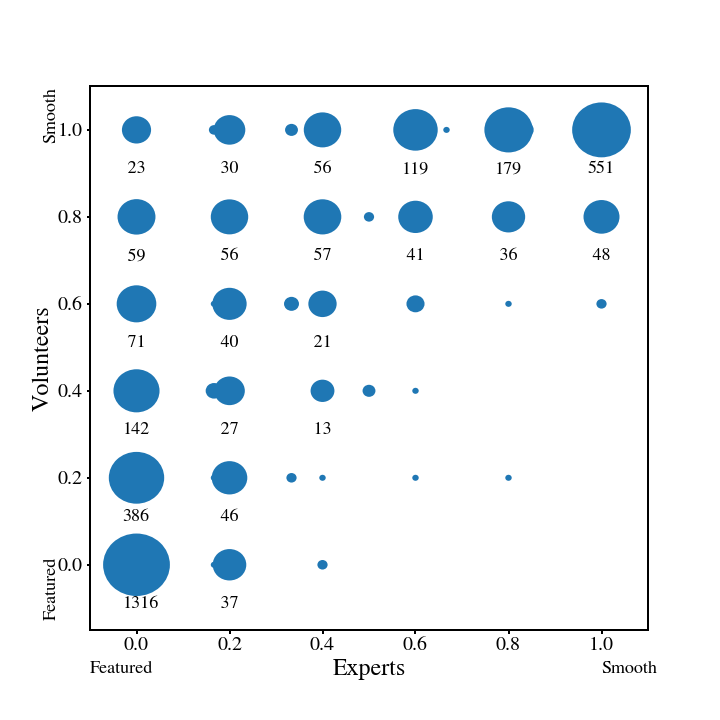
\includegraphics[width=5in]{Figures/expert_vs_volunteer_votes_highskill_11-6-17.png}
\caption[]{Volunter bias of labeling galaxies `Smooth' (\notfeat) as compared to expert classifications for the gold standard sample.}
\label{fig: volunteer bias}
\end{figure}

By comparing expert and GZ2 volunteer votes we uncover indications of volunteer bias towards labeling galaxies as `Smooth' (`Not Featured'). For each galaxy in our gold standard sample we identify the five most skilled volunteers who classified that galaxy, where skill is determined by the volunteer confusion matrix in Figure \ref{fig: confusion matrix}. We compute \fsmooth~from those five volunteers. In Figure \ref{fig: volunteer bias} we plot the volunteer \fsmooth~against the expert \fsmooth~sample, where the size of the circle is proportional to the number of subjects wherein both volunteers and experts agreed. Circles representing more than ten gold standard subjects are also labelled with the correponding number of galaxies at that location in \fsmooth~space. For example, there are 1316 subjects that both experts and volunteers labeled \feat~with \fsmooth~$ = 0.0$. Though the vast majority of galaxies received five expert classifications, some received more than that resulting in blue circles at one sixth intervals instead of the majority at fifths. The large circles at $0.0$ and $1.0$ indicate that both experts and volunteers agree for more than half of the gold standard sample. However, that the circles extend almost solely into the upper left hand corner indicates that volunteers consistently label galaxies as `Smooth' moreso than experts. Of this small sample, 40\% of galaxies are given a larger \fsmooth~by volunteers than by experts. 

It is well known that redshift and surface brightness affect the apparent strength of morphological features in CCD imaging in that finer details are harder to identify. GZ2 mitigate these issues by ``debiasing'' volunteer vote fractions \citep{Willett2013}. We compare both the original raw and debiased \fsmooth~vote fractions for the gold standard sample and find that it cannot account for the pronounced bias seen here. The reason for this is unsurprising as this sample was selected from the \cite{NairAbraham2010} catalog, which consists of bright, low-redshift galaxies. Effects due to cosmic distance are thus minor. 

This then suggests that the bias could be inherent to the question posed to volunteers: ``Is the galaxy simply smooth and rounded, with no sign of a disk?'' Terminology such as ``disk'' could be misinterpreted by those without specific astrophysics training. Experienced astronomers are more adept at identifying galactic disks, even those which posses few other obvious features. On the other hand, if volunteers do not see obvious features such as spiral arms or a bar, they could well mark galaxies as ``smooth.''  A similar issue is also observed in the GZ: CANDELS project in which \cite{Simmons2017} compares volunteer classifications to expert classifications collected by the CANDELS team \citep{Kartaltepe2015}. This comparison is, however, not ideal as the question posed to the CANDELS team was not identical to that given to GZ volunteers. With the small sample presented here, it is difficult to determine how much this bias could affect the full GZ2 galaxy sample though we touch on this issue again in Chapter \ref{chap:4}. 



%%----------------------------------------------------------------------------------------------------------------------------------------------------
%%   Subsection:    		SWAP only (FIDUCIAL RUN)
%%----------------------------------------------------------------------------------------------------------------------------------------------------
\subsection{Fiducial SWAP simulation}\label{sec: fiducial}

%% ----------------------------------------------------------------------------
%%   FIGURE:  VOLUNTEER PROBABILITIES
%% ----------------------------------------------------------------------------
\begin{figure}
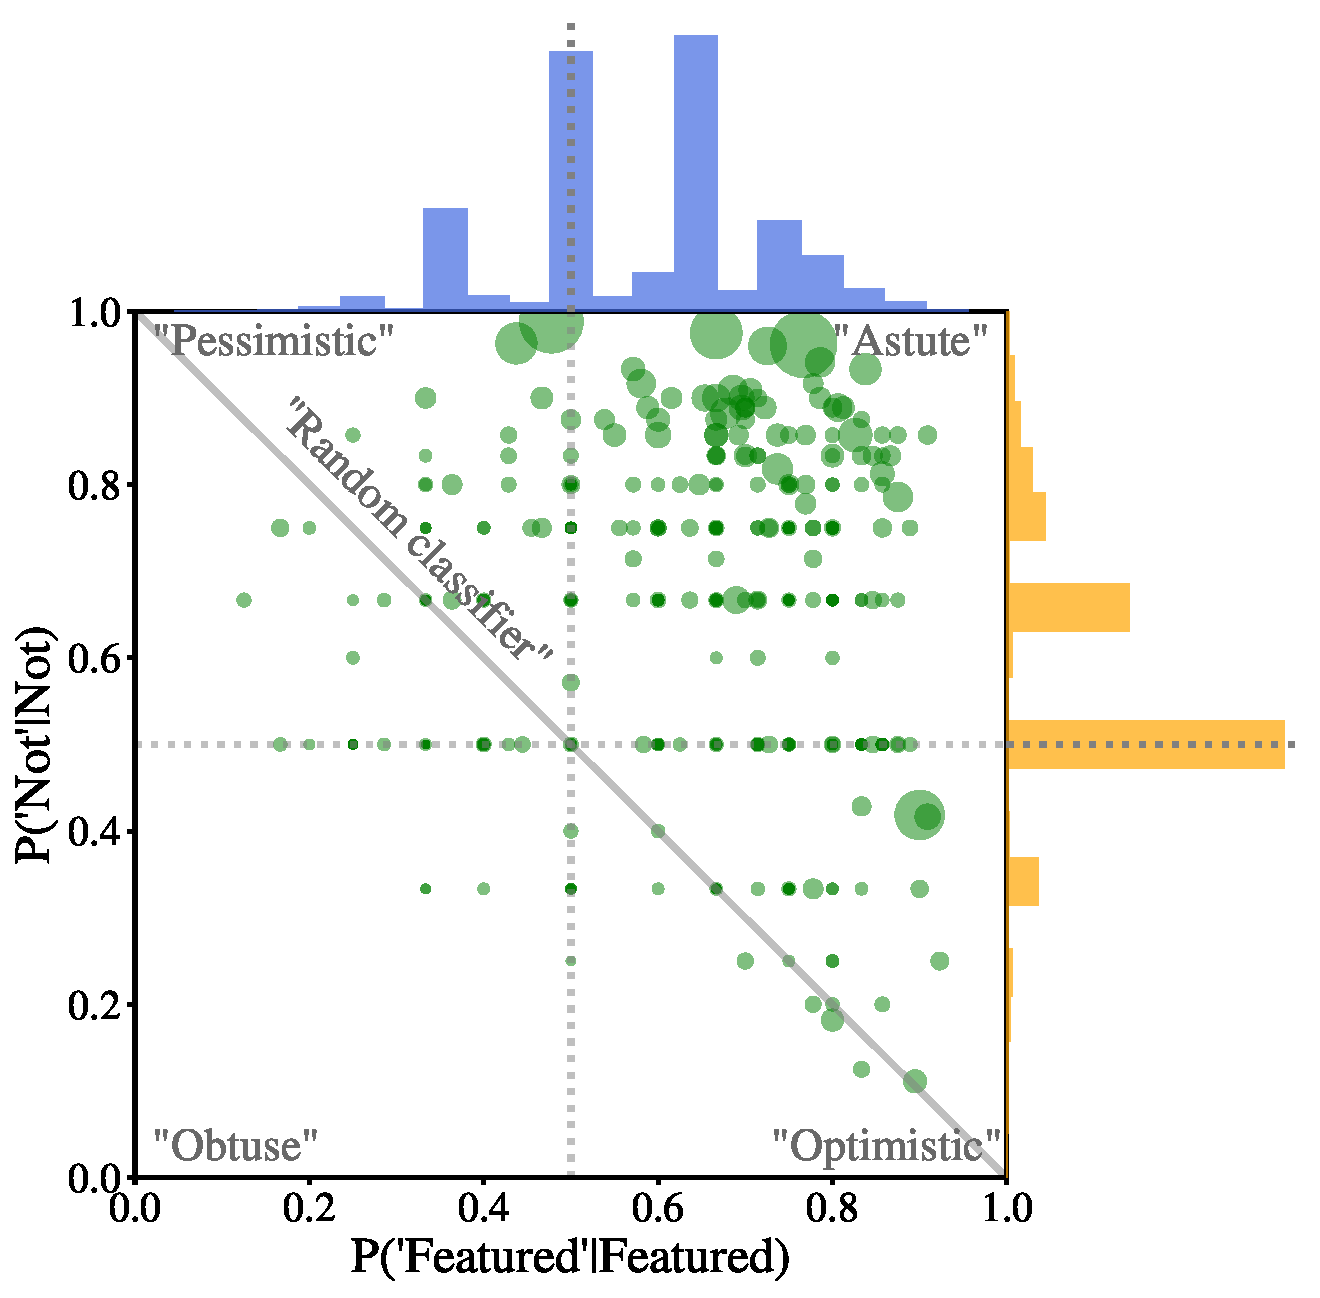
\includegraphics[width=3.45in]{Figures/human_machine/f2.pdf}
\caption[Volunteer confusion matrices achieved through SWAP reprocessing of GZ2 data.]{Confusion matrices for 1000 randomly selected GZ2 volunteers after fiducial SWAP assessment. Circle size is proportional to the number of gold standard subjects each volunteer classified. The histograms on top and right represent the distribution of each component of the confusion matrix for all volunteers.  A quarter of GZ2 volunteers are ``Astute"; they correctly identify both \feat~and \notfeat~subjects more than 50\% of the time. The peaks at 0.5 in both distributions are due primarily to volunteers who see only one training image: only half of their confusion matrix is updated.}
\label{fig: volunteer training}
\end{figure}

%%%-------------------------------------------------------
%%%  FIGURE:   SUBJECT POSTERIOR PROBABILITIES
%%%-------------------------------------------------------
\begin{figure} 
\centering
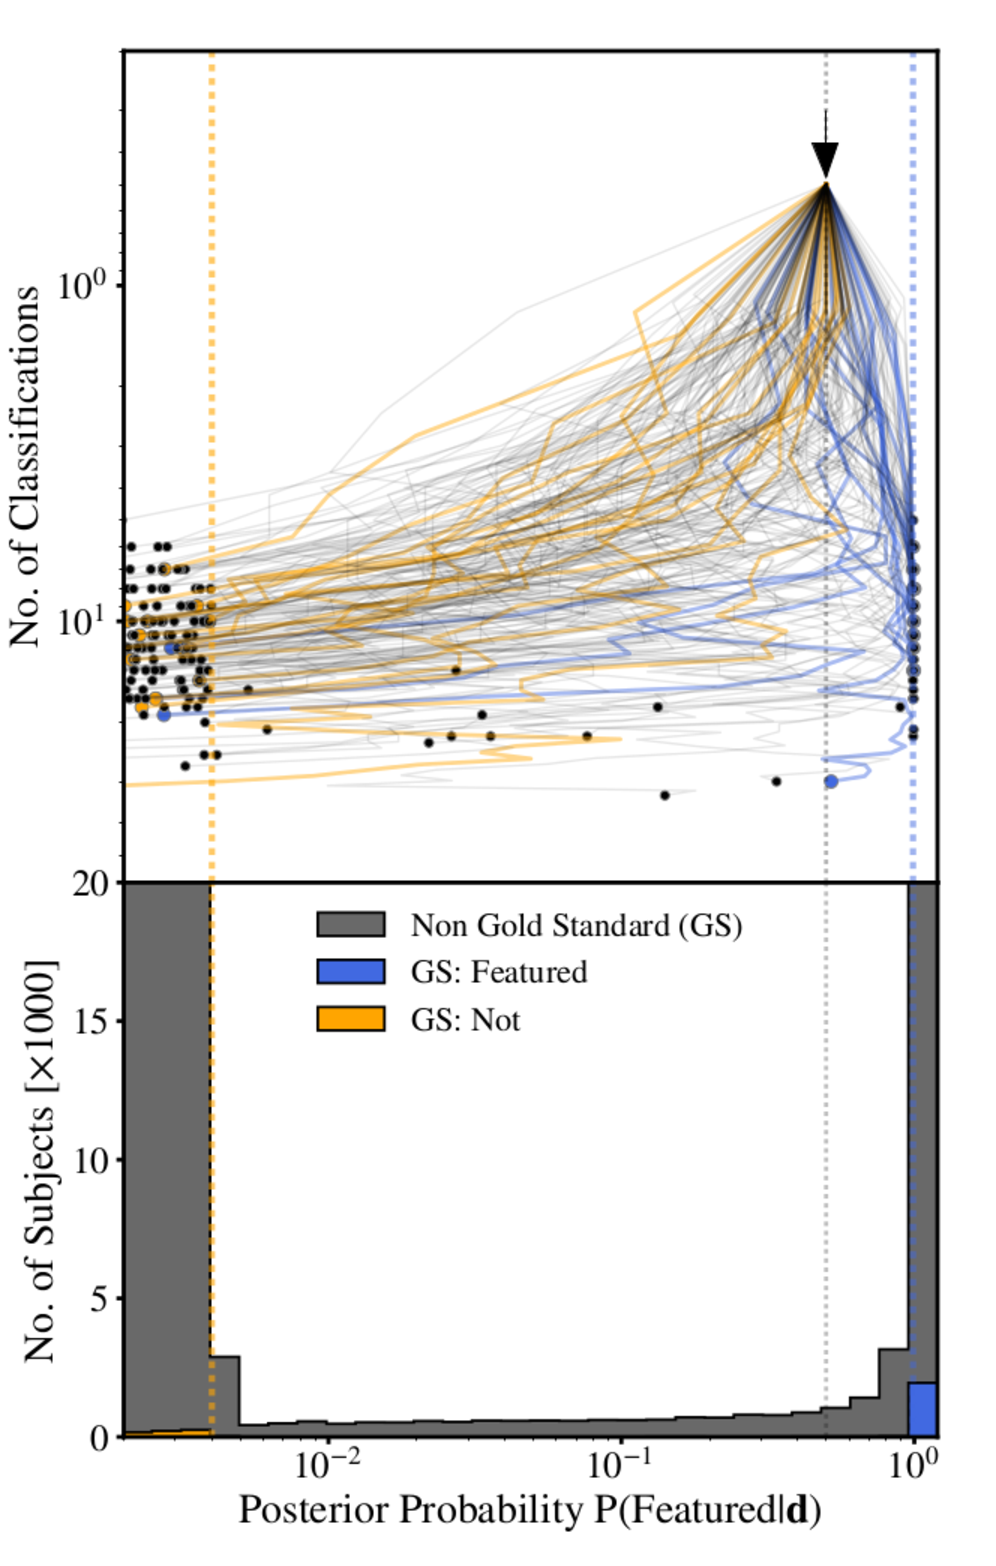
\includegraphics[width=3.25in]{Figures/human_machine/f12.pdf}
\caption[Galaxy posterior probabitilies realized through SWAP reprocessing of GZ2 data.]{Posterior probabilities for GZ2 subjects.  The top panel depicts the probability trajectories of 200 randomly selected GZ2 subjects. All subjects begin with a prior of 0.5 denoted by the arrow. Each subject's probability is nudged back and forth with each volunteer classification. From left to right the dotted vertical lines show the \notfeat~threshold, prior probability, and \feat~threshold. Different colours denote different types of subjects. The bottom panel shows the distribution in probability for all GZ2 subjects by the end of our simulation, where the y axis is truncated to show detail.}
\label{fig: subject probabilities}
\end{figure}


Before we run a simulation, a number of SWAP parameters must be chosen: the initial confusion matrix for each volunteer's agent, (\Pf, \Pn); the subject prior probability, \p; and the retirement thresholds, \tf~and \tn. For our fiducial  simulation, we initialize all confusion matrices at (0.5, 0.5), and set the subject prior probability, \p~$= 0.5$. We set the~\feat~threshold, \tf, i.e., the minimum probability for a subject to be retired as~\feat, to $0.99$. Similarly, we set the~\notfeat~threshold, \tn~$= 0.004$. In Section XXX we show that varying these parameters has only a small affect on the SWAP output. To simulate a live project, we run SWAP on a time step of $\Delta t = 1$ day, during which SWAP processes all volunteer classifications with timestamps within that range. This is performed for three months worth of GZ2 classification data. 

Figure~\ref{fig: volunteer training} (adapted from Figure 4 of~\citealt{Marshall2016}) demonstrates the volunteer assessment we achieve, and shows confusion matrices for 1000 randomly selected volunteers. The circle size is proportional to the number of gold standard subjects each volunteer classified. The histograms represent the distribution of each component of the confusion matrix for all volunteers. Nearly 25\% of volunteers are considered ``Astute"  indicating they correctly identify both \feat~and \notfeat~subjects more than 50\% of the time. Furthermore, as long as a volunteer's confusion matrix is different from random, they provide useful information to the project. The spikes at $0.5$ in the histograms are due to volunteers who see only one gold standard subject (i.e.,~\feat), leaving their probability in the other (\notfeat) unchanged. Additionally, 4\% of volunteers have a confusion matrix of (0.5, 0.5) indicating these volunteers classified two gold standard subjects of the same type, one correctly and one incorrectly. 

Figure~\ref{fig: subject probabilities} (adapted from Figure 5 of \citealt{Marshall2016}) demonstrates how subject posterior probabilities are updated with each classification. The arrow in the top panel denotes the prior probability, \p~$=0.5$. With each classification, that prior is updated into a posterior probability creating a trajectory through probability space for each subject. The blue and orange lines show the trajectories of a random sample of \feat~and \notfeat~subjects from our gold standard sample, while the black lines show the trajectories of a random sample of GZ2 subjects that were not part of the gold standard  sample. The similarly coloured vertical dashed lines correspond to the retirement thresholds, \tf~and \tn. The lower panel shows the full distribution of GZ2 subject posteriors at the end of our simulation, where the y-axis has been truncated to show detail. An overwhelming majority of subjects cross one of these retirement thresholds.

Our goal is to increase the efficiency of galaxy classification. We therefore  use as a metric the cumulative number of retired subjects as a function of the original GZ2 project time. We define a subject as GZ2-retired once it achieves at least 30 volunteer votes, encompassing 98.6\% of GZ2 subjects (explored in depth in Section XXX).  In contrast, a subject is considered SWAP-retired once its posterior probability crosses either of the retirement thresholds defined above. 

%%%-------------------------------------------------------
%%%  FIGURE:    CONFUSION MATRIX -- GZX VS GZ2
%%%-------------------------------------------------------
\begin{figure} 
\centering
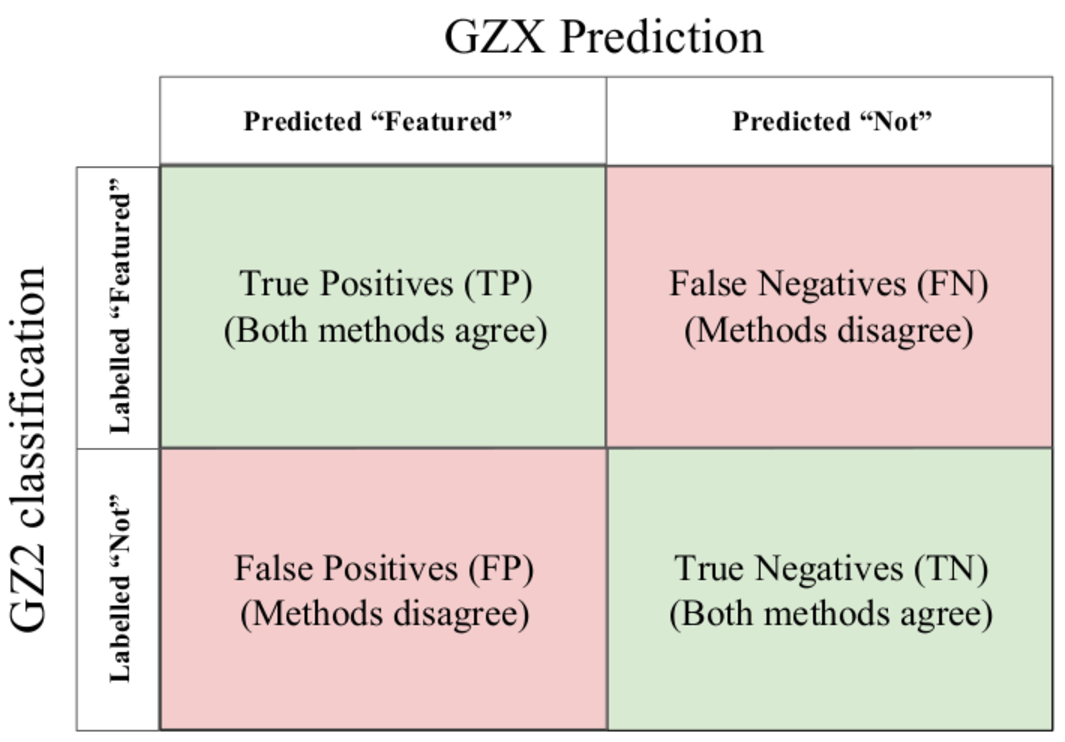
\includegraphics[width=3.2in]{Figures/human_machine/confusionmatrix.pdf}
\caption[Confusion matrix between predictions and ground truth defines quality metrics.]{Confusion matrix for comparing GZ2 classifications to our method.  True positives (TP) and true negatives (TN) indicate that the predictions from our method agree with GZ2 for subjects labelled \feat~and \notfeat, respectively. When the two classification methods disagree, the result is a sample of false negatives (FN) and false positives (FP). This allows us to easily compute  quality metrics like accuracy, completeness, and purity with respect to GZ2 as shown in Equations \ref{eqn: metrics}.} 
\label{fig: confusion matrix}
\end{figure}

However, it is important not to prioritize efficiency at the expense of quality. Because we have a binary classification we can construct a confusion matrix from which we can compute the quality metrics of accuracy, completeness and purity as a function of GZ2 project time by comparing our predicted labels to the \raw~labels. Figure \ref{fig: confusion matrix}
graphically depicts the elements of this confusion matrix. From this we compute: 
 
\begin{align*}\label{eqn: metrics}
\mathrm{accuracy} &= \frac{TP + TN}{TP + FP + TN + FN} \\
\mathrm{completeness} &= \frac{TP}{TP +FN }\tag{3} \\
\mathrm{purity} &= \frac{TP}{TP + FP}
\end{align*}

Thus, a complete sample recovers \textit{all} subjects labelled \feat~by GZ2, whereas a pure sample recovers \textit{only} subjects labelled \feat~by GZ2. For example, by Day 20, SWAP retires 120K subjects with 96\% accuracy, 99.7\% completeness, and 92\% purity. 
 
Figure \ref{fig: fiducial run} and Table~\ref{tab: summary} detail the results of our fiducial SWAP simulation compared to the original GZ2 project. The bottom panel shows the cumulative number of retired subjects as a function of GZ2 project time. By the end of our simulation, GZ2 (dashed dark blue) retires $\sim$50K subjects while SWAP (solid light blue) retires 226,124 subjects. We thus classify 80\% of the entire GZ2 sample in three months. Processing volunteer classifications through SWAP presents nearly a factor of 5 increase in classification efficiency. The top panel of Figure~\ref{fig: fiducial run} demonstrates the quality of those classifications as a function of time and establishes that our full SWAP-retired sample is 95.7\% accurate, 99\% complete, and 86.7\% pure. We discuss these small discrepancies in Section XXX.

%%%-------------------------------------------------------
%%%  FIGURE:    SWAP FIDUCIAL RUN
%%%-------------------------------------------------------
\begin{figure}
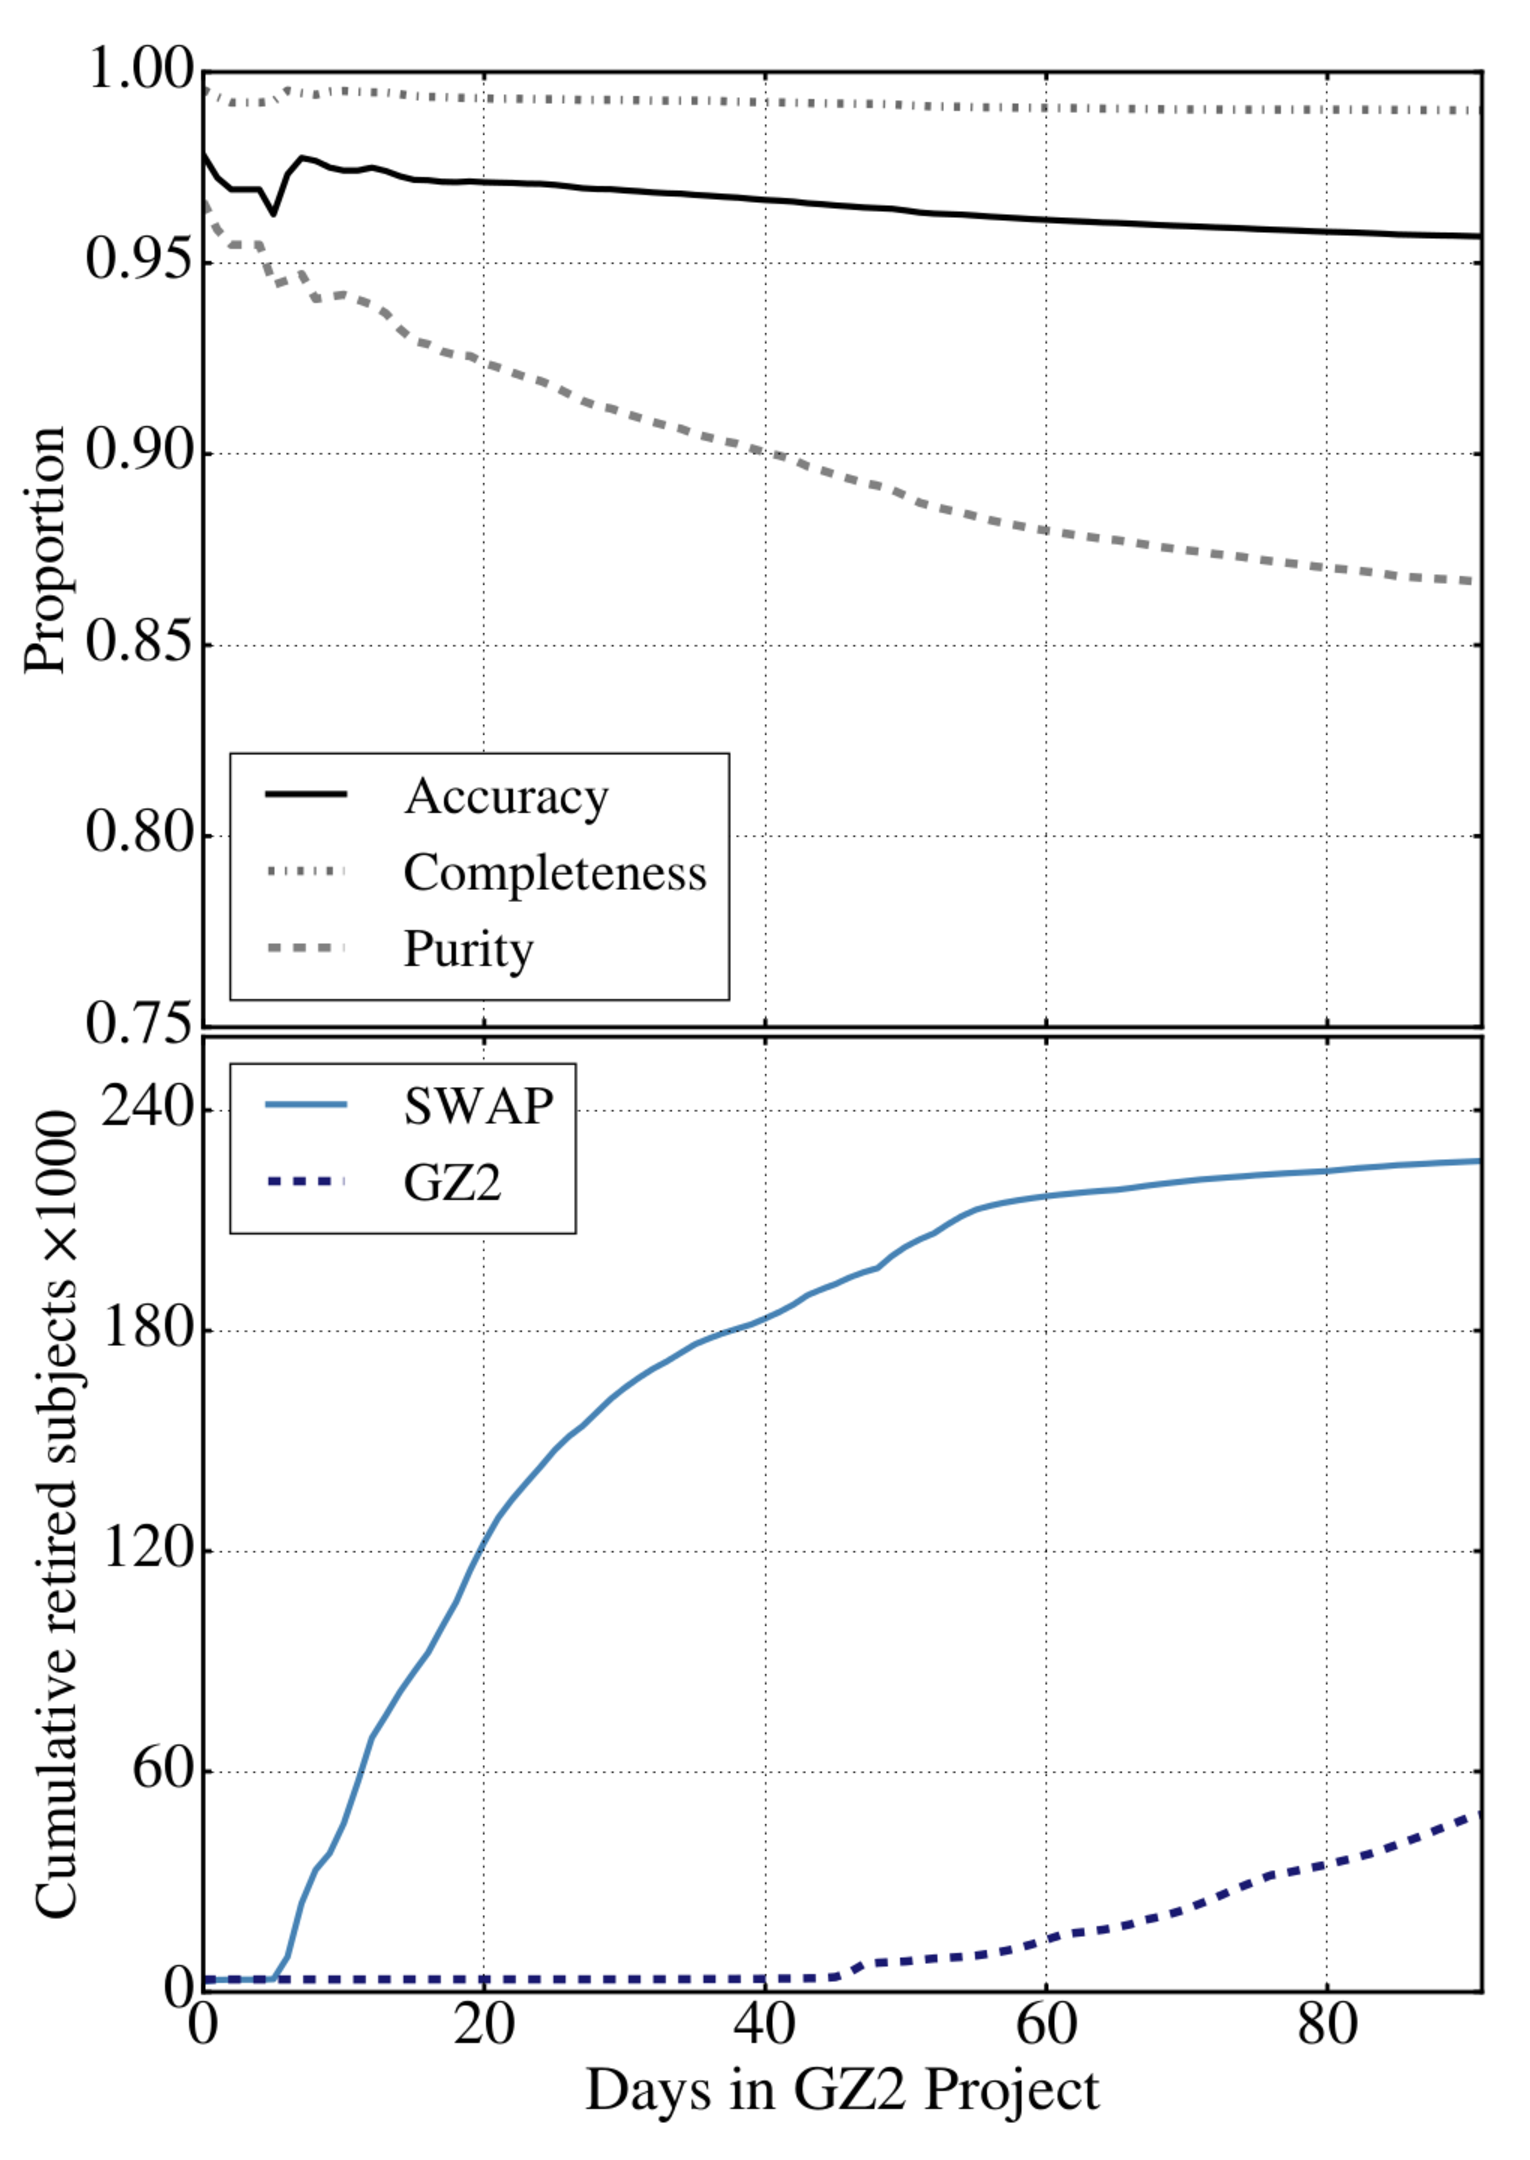
\includegraphics[width=3.35in]{Figures/human_machine/f3.pdf}
\caption[Reprocessing GZ2 data with SWAP results in a factor of increase in the classification rate.]{Fiducial SWAP simulation demonstrates a factor of 4.7 increase in the rate of subject retirement as a function of GZ2 project time (bottom panel, light blue) compared with the original GZ2 project (dashed dark blue). After 92 days, SWAP retires over 226K subjects, while GZ2 retires $\sim$48K.  The top panel displays the quality metrics (greys). These are calculated by comparing labels predicted by SWAP to~\raw~labels (Section~\ref{sec: data}) for the subject sample retired by that day of the simulation. Thus, on the final day, SWAP retires 226,124 subjects with 95.7\% accuracy,  and with completeness and purity of~\feat~subjects at 99\% and 86.7\% respectively. The decrease in purity as a function of time is due, in part, to the fact that more difficult to classify subjects are retired later in the simulation (see Section~\ref{sec: swap is faster}).}
\label{fig: fiducial run}
\end{figure}


%%%--------------------------------------------------------------------------------------------------
%%%  SECTION:   SWAP IS FASTER THAN GZ2 SANS DECISION TREE
%%%--------------------------------------------------------------------------------------------------
\subsection{Intelligent subject retirement}\label{sec: swap is faster}

That SWAP achieves a classification rate nearly 5 times faster than GZ2 comes with a caveat: we consider only the top-level question of the GZ2 decision tree, which, it can be argued, required that GZ2 secure enough votes to populate the subqueries.  In order to put SWAP and GZ2 on equal footing we determine the minimum number of votes, $N$, that the GZ2 project would need to achieve the same top-level classification for 95\% of its sample.

\begin{figure}
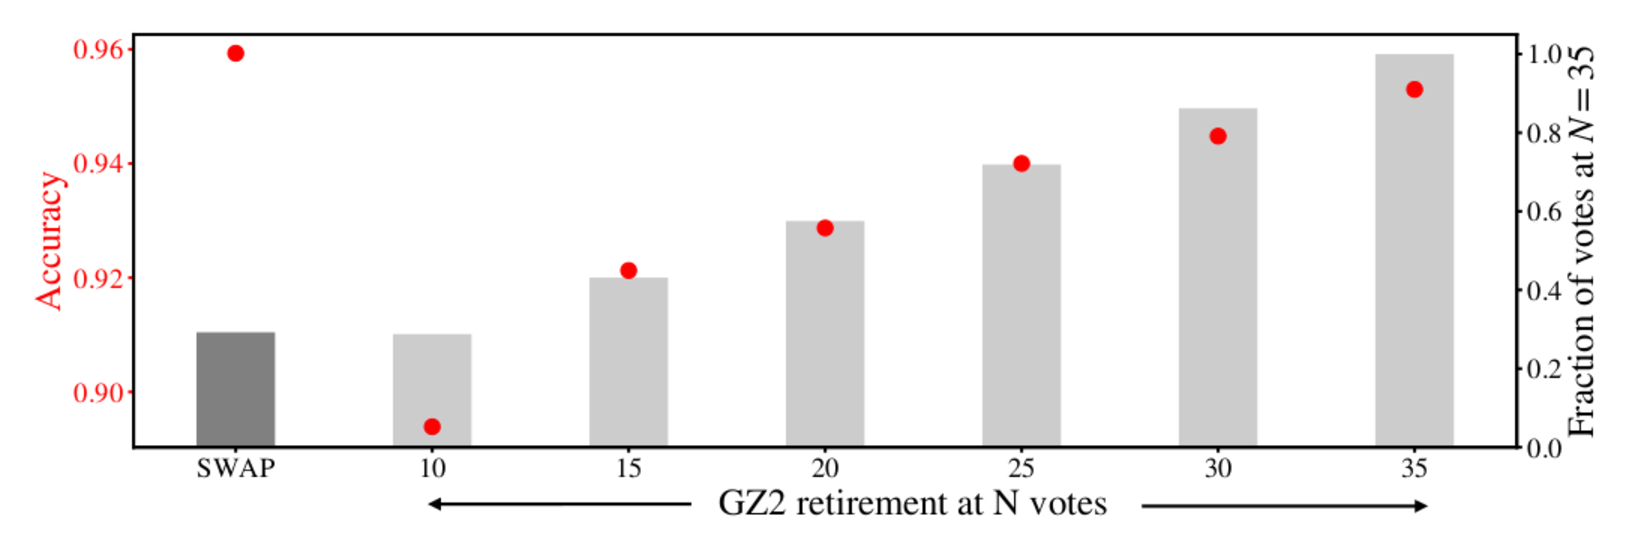
\includegraphics[width=\linewidth]{Figures/human_machine/f15.pdf}
\caption[SWAP's intelligent retirement mechanism 3.5 times fewer classifications than GZ2.]{SWAP's intelligent retirement mechanism allows it to use 30\% fewer classifications than GZ2 for the top-level question. To see this, we determine the minimum number of votes GZ2 needs in order to achieve consistent top-level classifications 95\% of the time, allowing us to compare the total number of votes in our SWAP simulation to the total number required for GZ2. We compute the vote fractions \fsmooth, \ffeat, and \fstar~using only the first $N$ votes in GZ2 and then compute the resulting class label.  We compare these labels to those we originally computed in Section~\ref{sec: data} using the full GZ2 vote fractions and compute the accuracy and the total number of votes necessary for subject retirement. We do this for 100 randomly selected subsamples from GZ2 with the same number of subjects as retired during our SWAP simulation. The red dots show the average accuracy while the grey bars denote the average fraction of votes compared to that required for $N=35$ (statistical error bars on these quantities are too small to be seen.) GZ2 needs at least 35 votes per subject in order to retain consistent subject classifications for 95\% of the GZ2 sample. SWAP can surpasses this accuracy using only 30\% as many votes.}
\label{fig: gz2 min retirement}
\end{figure}

We compute the raw vote fractions (\ffeat, \fsmooth, and \fstar) for every subject in the GZ2 sample using only the first $N$ classifications for $N \in [10, 15, 20, 25, 30, 35]$. From this, we compute descriptive labels as described in Section~\ref{sec: data}. Because our SWAP simulation did not retire every subject in the GZ2 sample, we select 100 random subsamples each consisting of 226,124 subjects, and compute the average accuracy and the average number of total GZ2 classifications necessary retire that subsample. These results are shown in Figure~\ref{fig: gz2 min retirement} for each value of $N$ along with the accuracy and total classifications for our SWAP simulation. We see that GZ2 needs at least 35 votes per subject in order to achieve consistent class labels 95\% of the time.  SWAP achieves the same accuracy with 30\% fewer classifications. Furthermore, this justifies our choice of defining a subject as GZ2-retired once it reached at least 30 classifications.

SWAP's performance can be explained through its retirement mechanism. GZ2 retired subjects randomly and required an arbitrary number of classifications per subject. In contrast, SWAP retires ``easier" subjects first while harder subjects remain in the system for longer (requiring many more classifications to nudge that subject's posterior across a retirement threshold).  Evidence for this can be seen in the top two panels of Figure~\ref{fig: swap retirement}. The top left panel shows the distribution of \fsmooth~for the entire GZ2 sample (orange), the SWAP-retired sample (blue), and the sample of subjects which SWAP has not yet retired, of which there are $\sim 19$K at the end of our simulation. The SWAP-retired sample generally follows the same distribution as GZ2-full except for the noticeable dip around \fsmooth$=0.6$. In contrast, the SWAP-not-yet-retired sample peaks at \fsmooth$=0.6$. These subjects can be interpreted as being the most difficult to classify which can be understood intuitively: galaxies with \fsmooth~$\le 0.5$ are easily identified as having features, while galaxies with \fsmooth~$\ge 0.8$ are obviously elliptical.

 This is further corroborated in the top right panel which shows the distribution of the number of classifications a subject had at the time of retirement. The solid lines show this distribution from the original GZ2 project for the same subsamples as the top left panel. For comparison, the dashed line shows the number of classifications at retirement realized during our SWAP simulation. Again, we see that the SWAP-retired sample is representative of GZ2 as a whole. However, the distribution for the SWAP-not-yet-retired sample is skewed toward fewer total classifications. To understand this, consider the following: GZ2 served subject images at random with the  exception that, towards the end of the project, subjects with low numbers of classifications were shown at a higher rate to ensure that each galaxy had enough responses to accurately characterize the likelihood of the classification~\citep{Willett2013}. The median number of classifications was 44 with the full distribution shown in orange in the top right panel of Figure~\ref{fig: swap retirement}. Our SWAP simulation processes these classifications in the same order as the original project (with the exception that gold-standard subject classifications are processed first as described in Section~\ref{sec: training sample}). Because our simulations cycle through only 92 days of GZ2 data, there are three general scenarios for why a subject has not yet been retired through SWAP: 1) SWAP has seen only a few of the many classifications for a given subject and it is not yet enough to retire it, 2) SWAP has seen many of the classifications for a subject but that subject is difficult; if we ran the simulation longer to process the remaining GZ2 classifications, SWAP would eventually retire it, and 3) SWAP has seen most or all of the classifications for a subject but it is difficult and there are few or no remaining GZ2 classifications; without additional volunteer input, these subjects will never be retired by SWAP. It is this third category that skews the red distribution towards fewer GZ2 votes. These are difficult-to-classify subjects that have only 30 - 40 GZ2 classifications, all of which are processed by SWAP, but these subjects remain unretired.

We have demonstrated that SWAP retires subjects intelligently: quickly retiring easy-to-classify subjects while allowing those that are more difficult to collect additional classifications. SWAP thus needs 30\% as many votes to retire nearly 5 times as many subjects during the three months of GZ2 project time that we include in our simulation.


%%%-------------------------------------------------------
%%%  FIGURE:    SWAP IS FASTER; RETIRES EASIEST FIRST
%%%-------------------------------------------------------
\begin{figure}
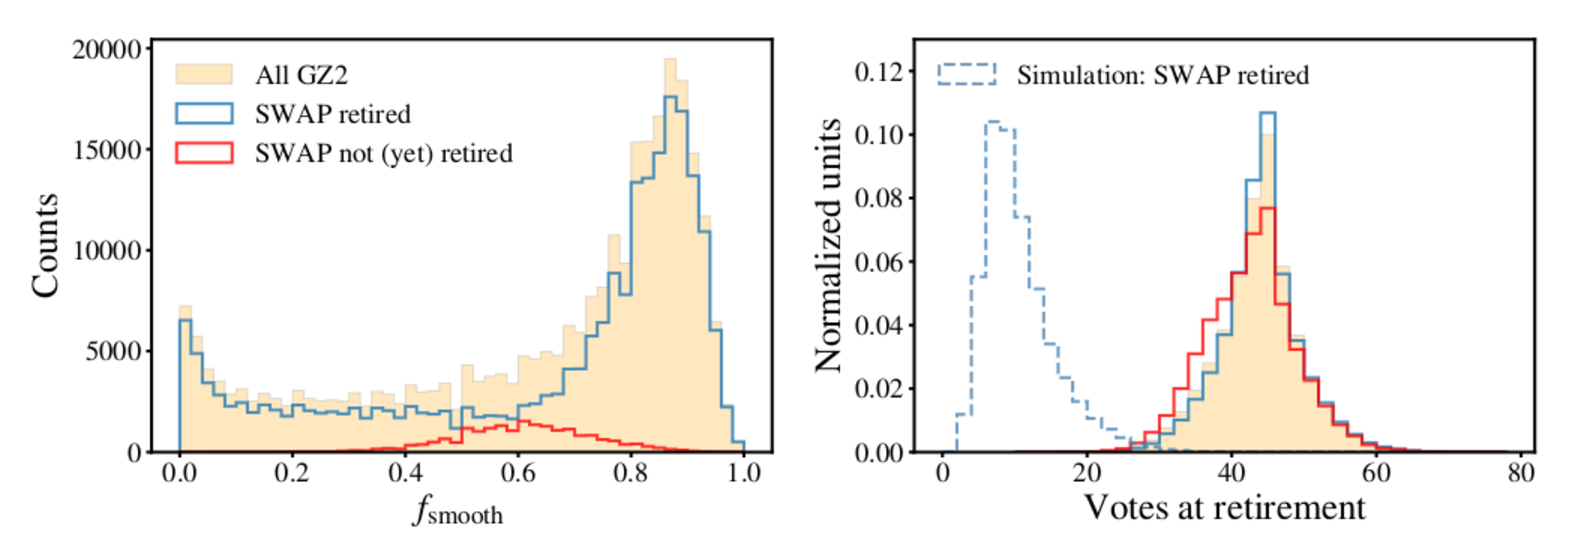
\includegraphics[width=\linewidth]{Figures/human_machine/f14.pdf}
\caption[SWAP increase classification efficiency by retiring ``easy'' galaxies quickly.]{SWAP uses 30\% fewer classifications to retire subjects due to its ability to retire easier subjects quickly, while more difficult subjects remain in the system to acquire additional classifications. The top left panel shows~\fsmooth~for the entire GZ2 sample (orange), the subjects retired by SWAP (blue), and subjects that SWAP has not yet retired by the end of our simulation (red). The latter distribution peaks at \fsmooth~$\sim 0.6$, which can intuitively be understood as the most difficult to classify subjects: those with \fsmooth~$\le 0.5$ are easily identified as \feat, while those with \fsmooth~$\ge 0.8$ are more obviously \notfeat. The top right panel provides additional evidence where here we show the number of votes at retirement for both the original GZ2 project (solid lines) and our SWAP simulation (dashed blue). The left-skew inherent in the red SWAP-not-yet-retired sample is due to difficult-to-classify subjects that received only 30-40 classifications during the GZ2 project. Even after processing all available classifications, SWAP cannot retire these subjects without additional volunteer input.}
\label{fig: swap retirement}
\end{figure}



\subsection{Reducing human effort}
SWAP's intelligent retirement mechanism is due, in large part, to how SWAP estimates volunteer classification ability which, in turn, allows for a dramatic reduction in the amount of human effort (votes) required. To see this, we consider a toy model wherein we simulate volunteers with fixed confusion matrices. We simulate 1000 \feat~subjects and 1000 \notfeat~subjects each with prior, \p~$ = 0.5$. We simulate 100 volunteer agents all with the same fixed confusion matrix of (0.63, 0.65), where these values are computed as the average \Pf~and \Pn~from our assessment of real volunteers, excluding the spikes at 0.5. We generate volunteer classifications based on this confusion matrix (i.e., volunteers will correctly identify \feat~subjects 63\% of the time) and update the subject's posterior probability with each classification. We track how many classifications are required for each subject's posterior to cross either the \feat~or \notfeat~retirement thresholds. 


%%%-------------------------------------------------------
%%%  FIGURE:   SWAP vote distributions
%%%-------------------------------------------------------
\begin{figure}
\centering
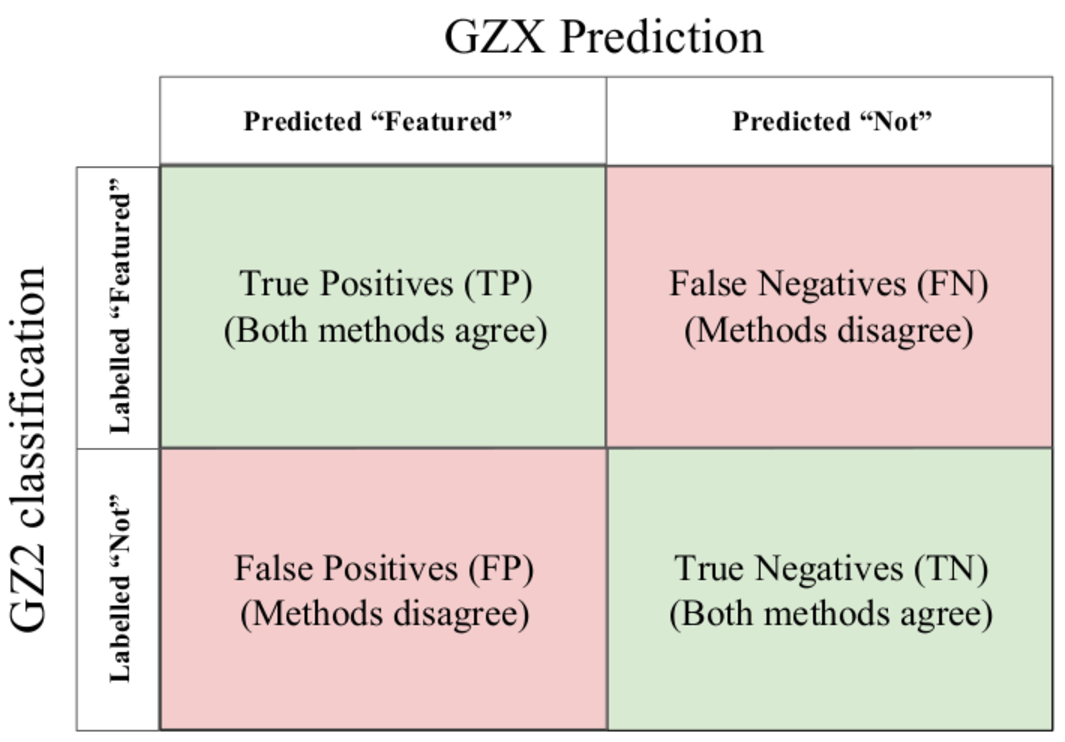
\includegraphics[width=3.5in]{Figures/human_machine/f4.pdf}
\caption[SWAP's volunteer-weighting mechanism provides a factor of three reduction in the required human effort for classification tasks.]{SWAP's volunteer-weighting mechanism provides a factor of three reduction in the human effort required to retire GZ2 subjects. The filled histograms show the number of volunteer classifications per subject achieved during our SWAP simulation broken down by class label, where the solid black line is the total. The dashed histograms are results from our toy model in which we simulate volunteers with fixed confusion matrices, effectively disengaging SWAP's volunteer-weighting mechanism. These broad distributions require $\sim$3 times more classifications per subject to reach the same retirement thresholds.} 
\label{fig: swap vote distributions}
\end{figure}

The results are presented in Figure~\ref{fig: swap vote distributions}. The filled blue and orange histograms show the number of classifications per subject achieved from our SWAP simulation, where volunteer agent confusion matrices are those from Figure~\ref{fig: volunteer training}. The dashed blue and orange distributions are the results from our toy model. When SWAP accounts for volunteer ability, most subjects are retired with between 6 and 15 votes, with a median of 9 votes. In contrast, when every volunteer is given equal weighting, subjects require 16 to 45 votes with a median of 30 votes before crossing one of the retirement thresholds. Thus the volunteer weighting scheme embedded in SWAP can reduce the amount of human effort required to retire subjects by a factor of three.

This reduction will be, in part, a function of the number of gold standard subjects each volunteer sees.  Our gold standard sample was chosen to be representative of morphology rather than evenly distributed among GZ2 volunteers. We thus find that half of our volunteers classify only one or two gold standard subjects. That we achieve a factor of three reduction when only half of our volunteer pool has seen $\ge 2$ gold standard subjects suggests that an additional reduction of  human effort is possible with more extensive volunteer training.



\subsection{Disagreements between SWAP and GZ2}\label{sec: swap gz2 disagree}

Galaxy Zoo's strength comes from the consensus of dozens of volunteers voting on each subject. Processing votes with SWAP reduces the number of classifications to reach consensus. Though we typically recover the \raw~label, SWAP disagrees about 5\% of the time. We thus examine the false positives (subjects SWAP labels as \feat~but \raw~labels as~\notfeat) and false negatives (subjects SWAP labels as \notfeat~but \raw~labels as \feat). We explore these subjects in redshift, magnitude, physical size, and concentration but find no correlation with any of these variables, suggesting that, at least for this galaxy sample, the reliability of morphology depends on factors that are not captured by these coarse measurements. This is perhaps unsurprising since GZ2 subjects were selected from the larger GZ1 sample to be the brightest, largest and nearest galaxies:  precisely those subjects most accessible for visual classification. 

%%%-------------------------------------------------------
%%%  FIGURE:   SWAP failures
%%%-------------------------------------------------------
\begin{figure}
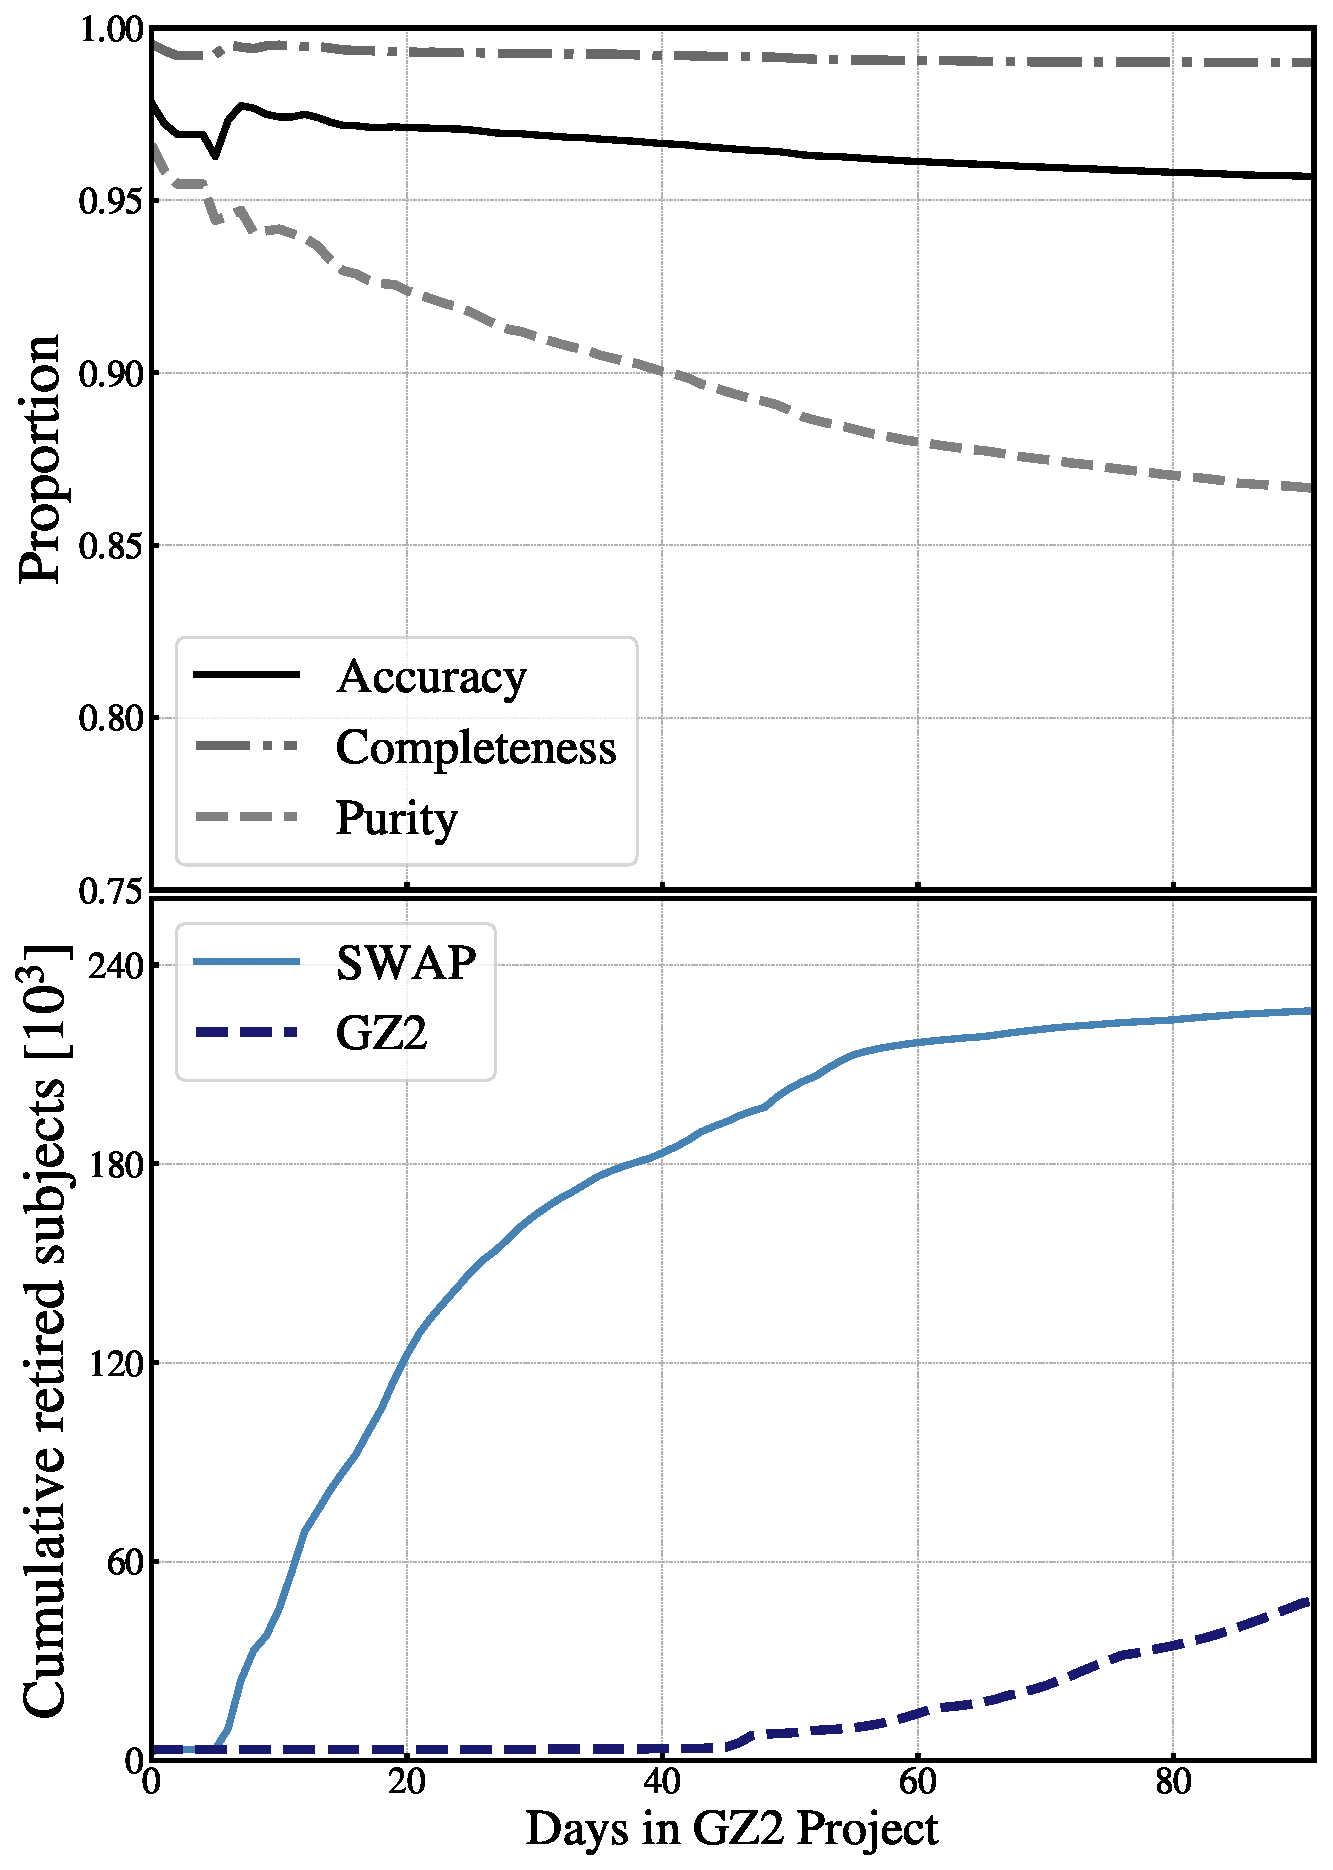
\includegraphics[width=3.5in]{Figures/human_machine/f5.pdf}
\caption[SWAP's prediction disagrees with the GZ2 label as a result of the confidence interval around the chosen threshold used to define the GZ2 label.]{Distribution of GZ2 \ffeat+\fstar~vote fractions for subjects correctly identified by SWAP (dotted grey), along with those identified as false positives (solid purple), and false negatives (dashed teal). 
The false positives and false negatives are scaled by factors of 10 and 100 respectively for easier comparison. From Section~\ref{sec: data}, subjects with values $> 0.5$ are defined as~\feat, however, the teal distribution indicates that SWAP labels them as~\notfeat. This is not a flaw of SWAP: 68.9\% of incorrectly identified subjects have $0.4 \le $~\ffeat +\fstar~$ \le 0.6$ suggesting that~\raw~labels are simply too uncertain. The overlap between the false positives and negatives is due to subjects that are exactly 50-50; by default these are labelled~\notfeat.}
\label{fig: SWAP sucks}
\end{figure}

Instead we consider the stochastic nature of GZ2 vote fractions, which can be estimated as binomial. Let success be a response of ``smooth'' and failure be any other response. The $68\%$ confidence interval on a subject with \fsmooth~$=0.5$ is then $(0.42, 0.57)$ assuming 40 classifications, each with a probability of 0.5. Figure~\ref{fig: SWAP sucks} shows the distribution of \ffeat+\fstar~for the false positives (solid purple), and the false negatives (dashed teal) compared to the  subjects where SWAP and GZ2 agree (dotted grey).  Recall that if this value is greater than 0.5, the subject is labeled \feat. The majority of disagreements between SWAP and GZ2 are for subjects that have $0.4 <$~\ffeat+\fstar~$< 0.6$. It is thus unsurprising that SWAP and GZ2 disagree most within the approximate confidence interval of our selected GZ2 threshold. We note that the distribution overlap between false positives and false negatives is due to subjects that do not have a majority; these are labeled \notfeat~by default. 

Two other effects contribute to the disagreement between SWAP and GZ2. First, as the number of classifications used to retire a galaxy decreases, the likelihood of misclassification by random chance increases. Second, disagreement arises due to expert-level volunteers whose confusion matrices are close to 1.0. These volunteers are essentially more strongly weighted, allowing that subject's posterior to cross a retirement threshold in as few as two classifications. In rare cases, despite training, some expert-level 
volunteers get it wrong compared to the gold-standard labels. These issues can be mitigated by requiring each subject reach a minimum number of classifications in addition to its posterior probability crossing a retirement threshold, thus combining the best qualities of GZ2 and SWAP. 


\subsection{Summary}

%In Appendix~\ref{sec: tweaking swap}, we find that varying the initial SWAP 
%parameters from the fiducial values does not substantially change the results 
%presented here. The largest influence comes from choosing unrealistic subject 
%prior probabilities, which can mildly degrade the quality of the resulting classifications. 
%More importantly, none of these effects significantly alters our human and machine integration in Section~\ref{sec: results}. 


We demonstrate nearly a factor of five increase in the classification rate, a reduction of at least a factor of three in the human effort necessary to maintain that increased rate, all while maintaining 95\% accuracy, nearly perfect completeness of~\feat~subjects, and with a purity that can be controlled by careful selection of input parameters to be better than 90\% (see Appendix~\ref{sec: tweaking swap}). Exploring those subjects wherein SWAP and GZ2 disagree, we conclude that the majority of this disagreement stems from the stochastic nature of~\raw~labels. We now turn our focus towards incorporating a machine classifier utilizing these SWAP-retired subjects as a training sample. 


%% ------------------------------------------------------------------------------------------------------------------------------
%% 		EXPLORING SWAP PARAMETERS
%% ------------------------------------------------------------------------------------------------------------------------------
\section{Exploring SWAP's Parameter Space} \label{sec: tweaking swap}

The entirety of our analysis thus far has assumed the most basic SWAP parameters. In this section we explore how SWAP's classification output changes as a function of varying the initial agent confusion matrices, prior probability, and retirement thresholds.


\subsection{Initial agent confusion matrix.} 
In our fiducial simulation each volunteer was assigned an agent whose confusion matrix was initialized at $(0.5, 0.5)$, which presumes that volunteers are no better than random classifiers. We perform two simulations wherein we initialize agent confusion matrices as $(0.4, 0.4)$, slightly obtuse volunteers; and $(0.6, 0.6)$, slightly astute volunteers, with everything else remaining constant.  Results of these simulations compared to the fiducial run are shown in the left panel of Figure~\ref{fig: tweak swap}. We find that SWAP is largely insensitive to the initial confusion matrix  both in terms of the subject retirement rate and classification quality.  

%% -------------------------------------------------------------------------------
%%   FIGURE:  SWAP --  CONFUSION MATRIX & PRIOR 
%% -------------------------------------------------------------------------------
\begin{figure*}
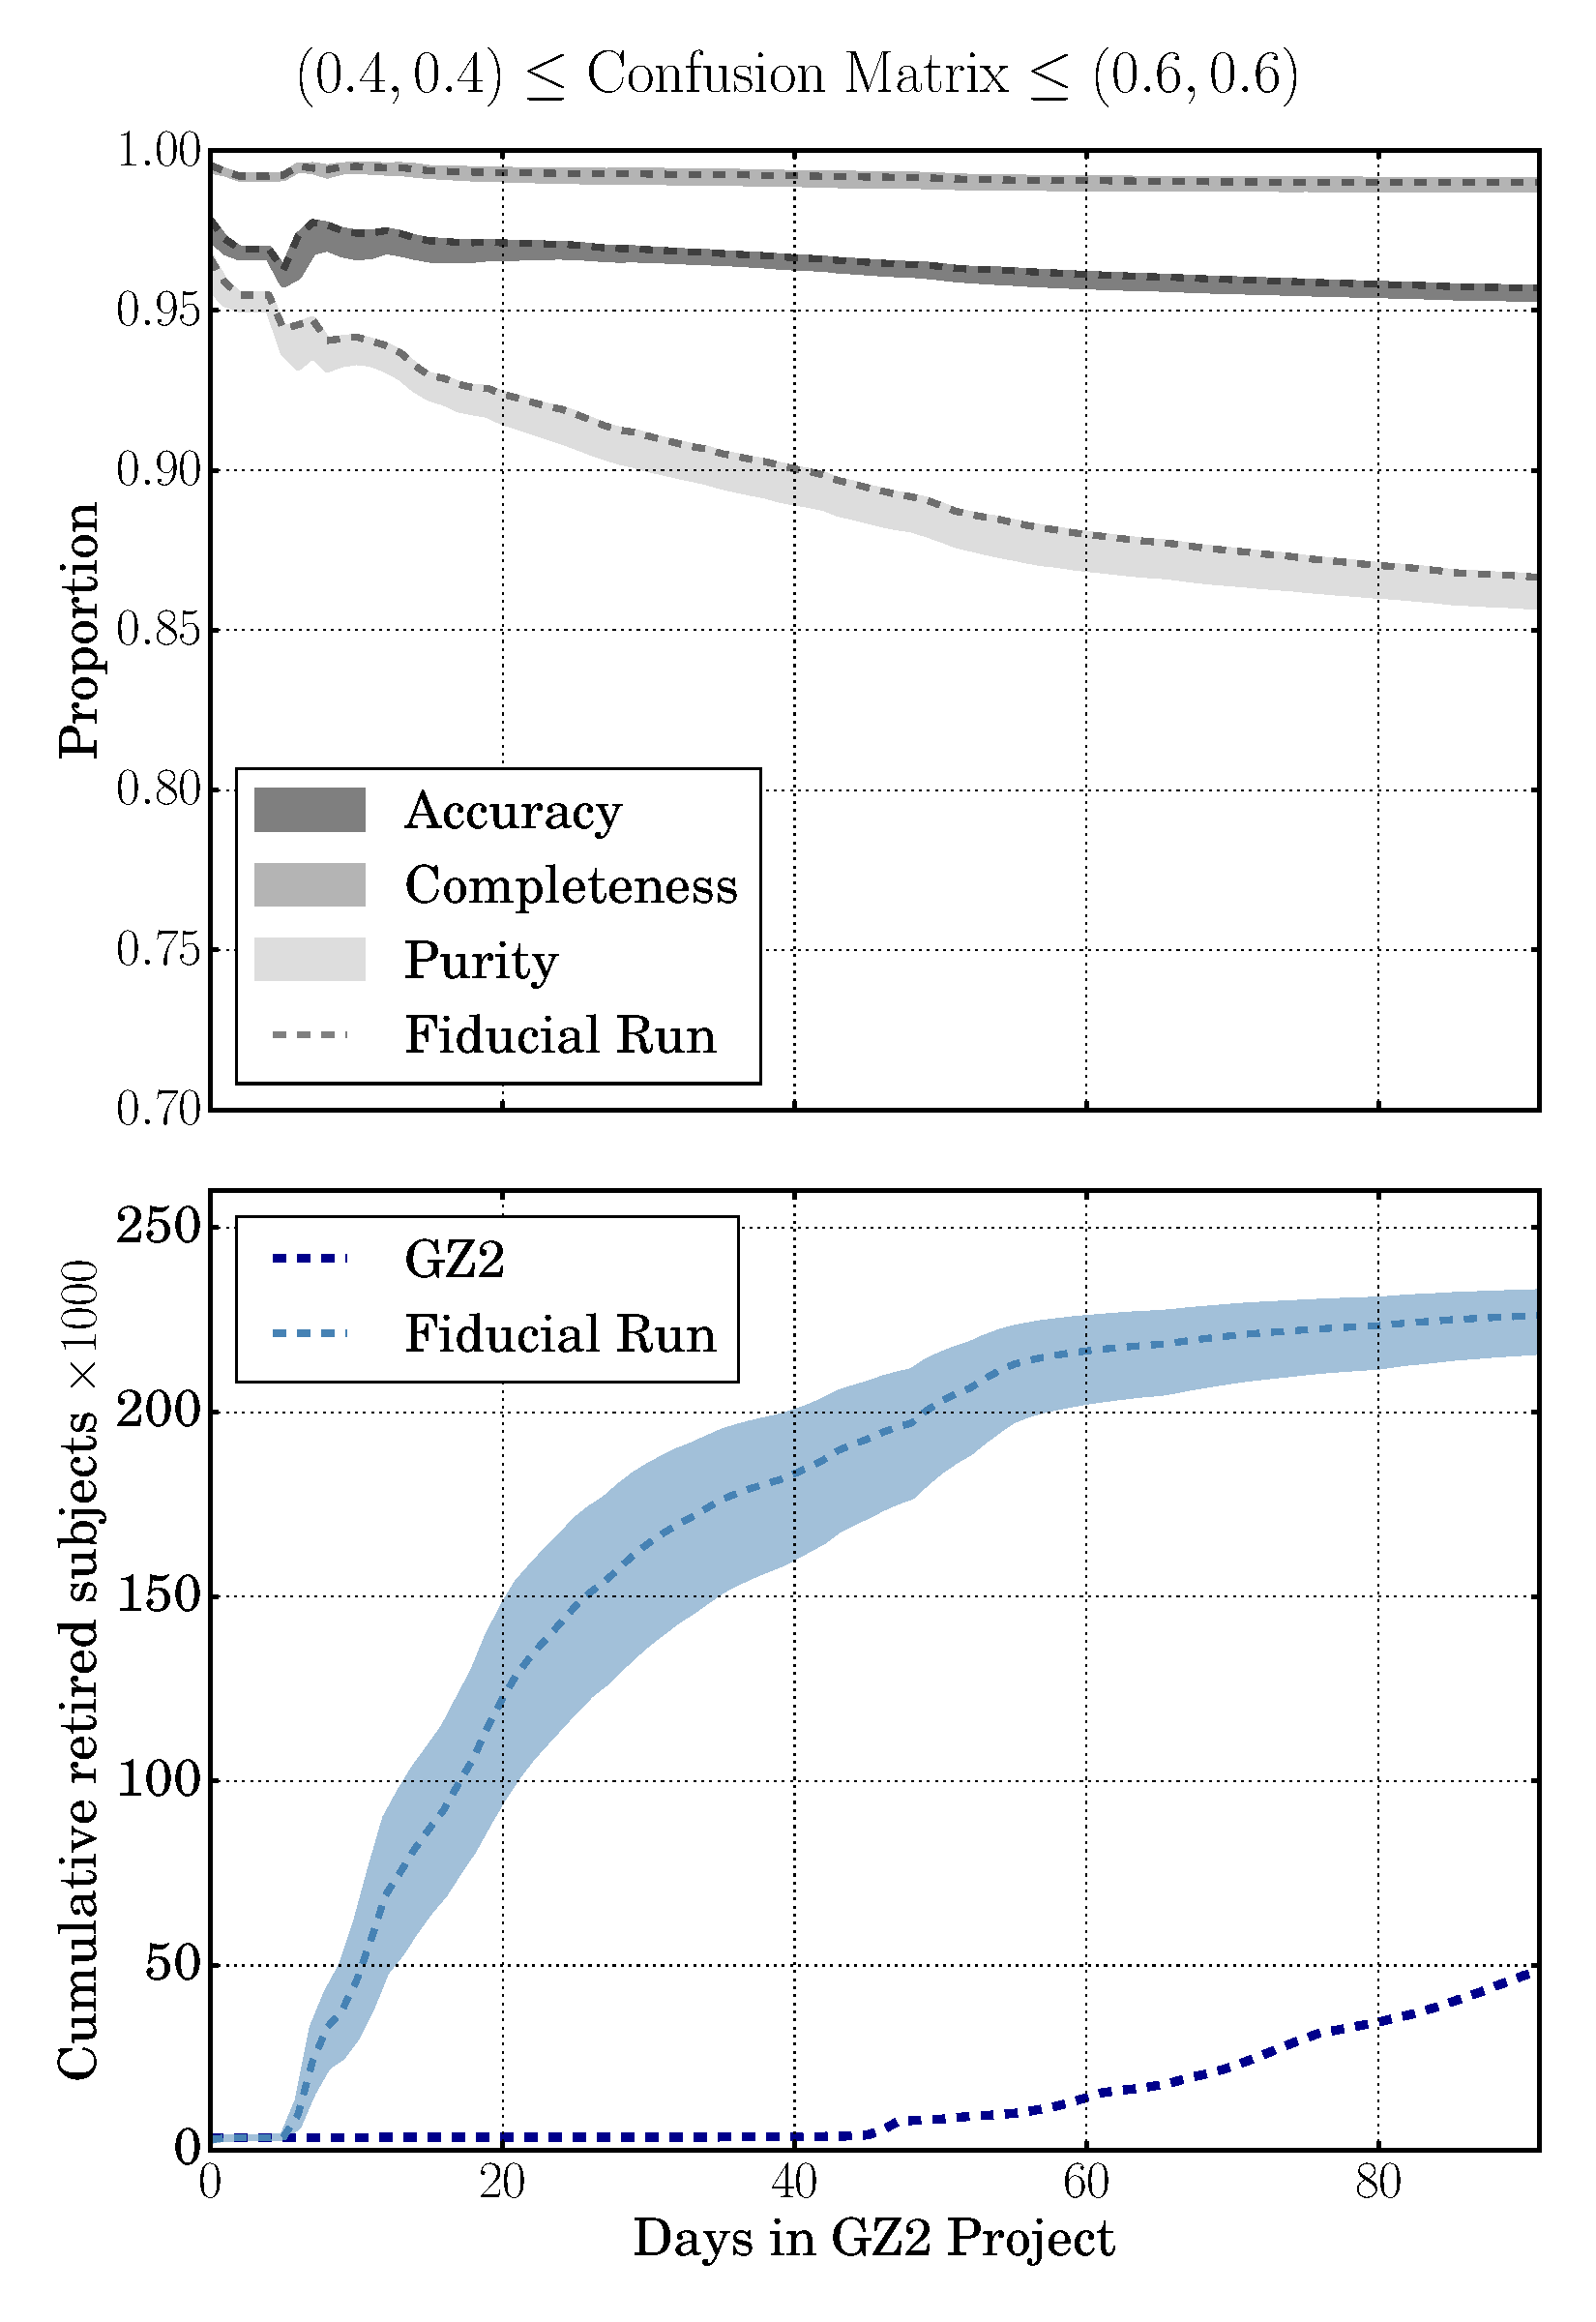
\includegraphics[width=2.8in]{Figures/human_machine/A1a.pdf}
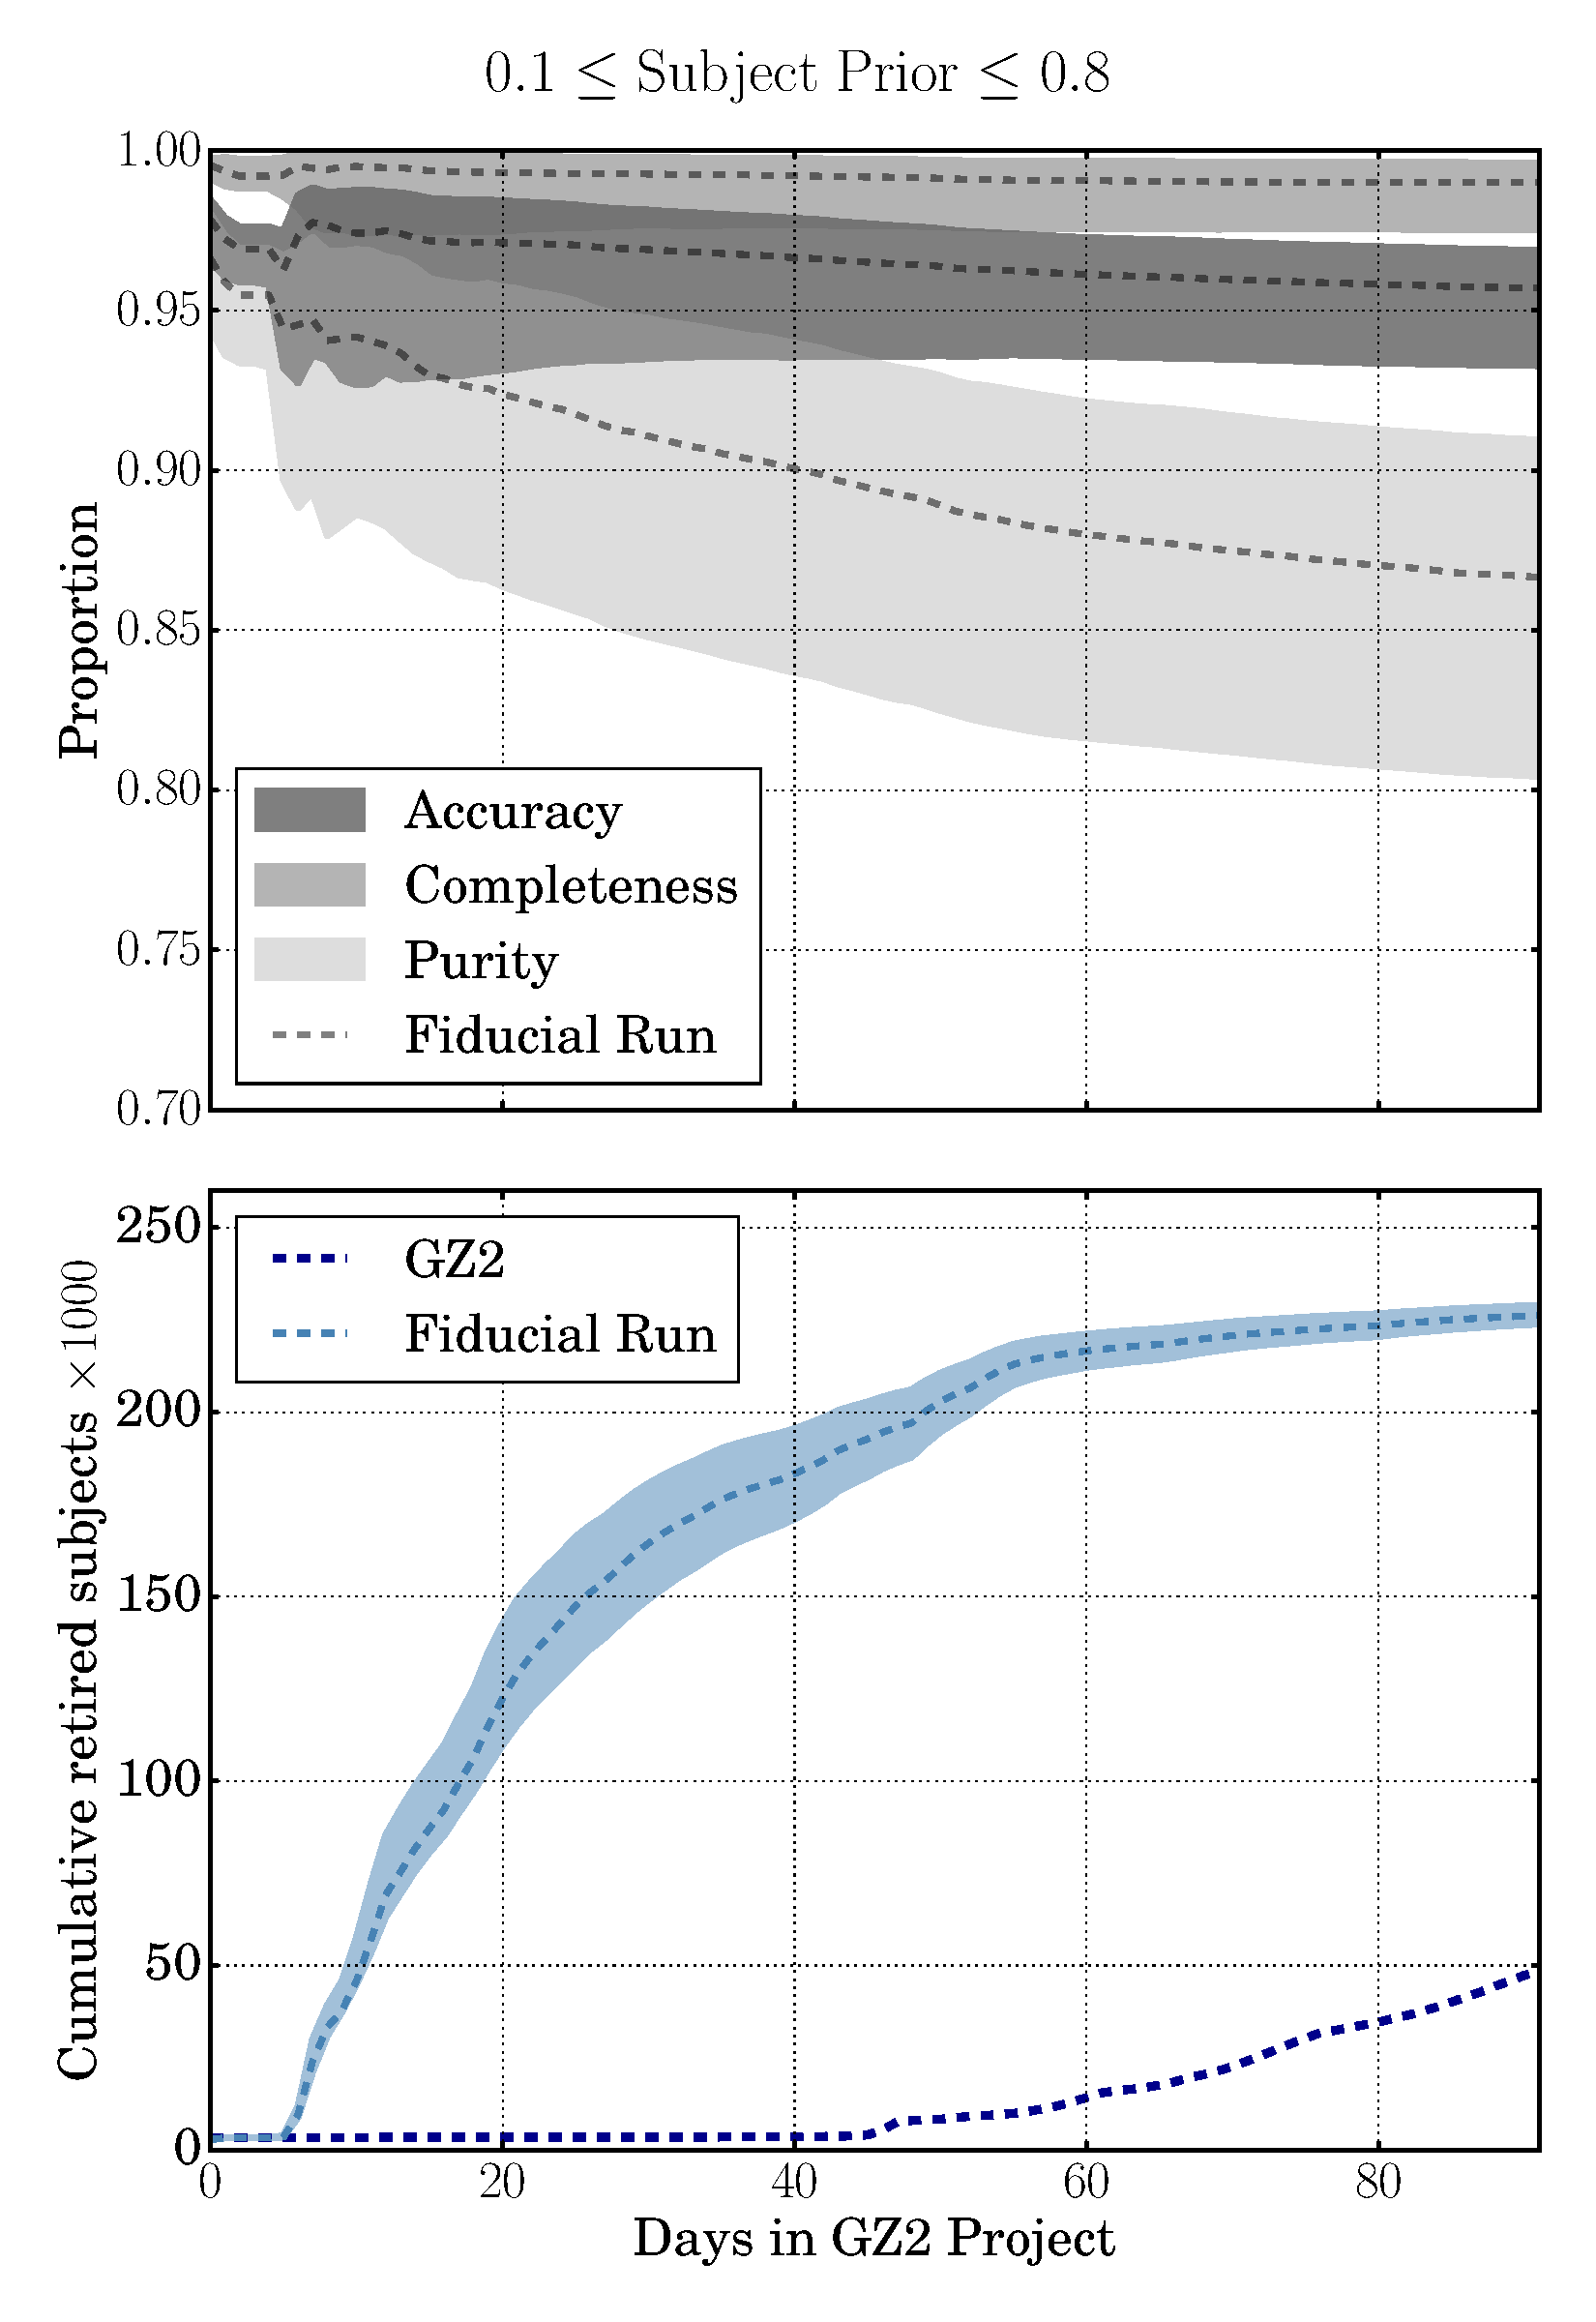
\includegraphics[width=2.8in]{Figures/human_machine/A1b.pdf}
\caption[SWAP's performance is robust to changes in initial volunteer confusion matrix and subject prior.]{SWAP performance does not dramatically change even with a range of input parameters (shaded regions) as compared to the fiducial run of Section~\ref{sec: fiducial} (dashed lines).  \textit{Left.} The quality (top) and retirement rate (bottom) when the confusion matrix is initialized as (0.4, 0.4) and (0.6, 0.6), with all other input parameters remaining constant. \textit{Right.} Same as the left panel but allowing the subject prior probability, \p $= 0.2, 0.35$ and $0.8$. Changing the confusion matrix has little impact on the quality of the labels but varies the total number of subjects retired. In contrast, changing the subject prior is more likely to affect the classification quality rather than the total number of subjects retired. \label{fig: tweak swap}}
\end{figure*}

We retire $\sim$$225$K$\pm3.5\%$ subjects as shown by the light blue shaded region in the bottom left panel of Figure~\ref{fig: tweak swap}, where the dashed blue line denotes the fiducial run. Predictably, when the confusion matrix probabilities are low, we retire fewer subjects than when these probabilities are high for a given period of time. This is easy to understand since it takes longer for volunteers to become astute classifiers when they are initially given values denoting them as obtuse. Regardless, most volunteers become astute classifiers by the end of the simulation. The top left panel demonstrates our usual quality metrics as computed in Section \ref{sec: fiducial}. The dashed lines again denote the fiducial run. We maintain $\sim$$95\%$ accuracy, $99\%$ completeness, and $\sim$$84\%$ purity;  and no metric changes by $> 2\%$ regardless of initial confusion matrix values.  
 
This spread is due to three effects: 
1) subjects can receive an alternate SWAP label in different simulations, 
2) subjects can be retired in a different order, and 
3) the set of retired subjects is not guaranteed to be common to all runs. 
We find SWAP to be highly consistent: more than 99\% of retired subjects are the same among all simulations, and, of these, 99\% receive the same label.  Instead we find that the order in which subjects are retired changes between runs. When the confusion matrix is low, subjects take longer to classify compared to the fiducial run (i.e., they retire on a later date in GZ2 project time). Likewise, subjects retire sooner when the confusion matrix is high. This can cause quality metrics to vary since they are calculated on a day to day basis. These effects each contribute less than one per cent variation and thus we see a high level of consistency between simulations. 

Of interest, perhaps, is that the quality metrics for these simulations are not symmetric about the fiducial run. However, in the Bayesian framework of SWAP, an agent with confusion matrix (0.4, 0.4) contributes as much information as an agent with confusion matrix (0.6, 0.6). The quality metrics computed are thus within a per cent of each other. In either case, we find that initializing agents at (0.5, 0.5) provides optimal performance for the `training' we simulate with our current approach. Further assessment would require a live project with real-time training and feedback. 


\subsection{Subject prior probability,~\p.}
The prior probability assigned to each subject is an educated guess of the frequency of that characteristic in the scope of the data at hand. For galaxy morphologies, this number should be an estimate of the probability of observing a desired feature (bar, disk, ring, etc.). In our case, we desire simply to find galaxies that are~\feat; however, this is dependent on mass, redshift, physical size, etc. The original GZ2 sample was selected primarily on magnitude and redshift.  As there was no cut on galaxy size (with the exception that each galaxy be larger than the SDSS PSF), the sample includes a large range of  masses and sizes. Designating a single prior is not clear-cut; we thus explore how various~\p~values effect the SWAP outcome.

We run simulations allowing~\p~to take values 0.2, 0.35, and 0.8 
and compare these to the fiducial run, with everything else remaining constant. The results are shown in the right panels of Figure~\ref{fig: tweak swap}. We again find that SWAP is consistent in terms of subject retirement which varies by only 1\%. However, as can be seen in the top panel, the variation in our quality metrics is more pronounced. Firstly, though we retire nearly the same number of subjects over the course of each simulation, they are less consistent than our previous runs. That is, only 95\% of retired subjects are common to all simulations. Secondly, of those that are common, only 94\% receive the same label from SWAP indicating that hanging the prior is more likely to produce a different label for a given subject than changing the initial agent confusion matrix. Finally, there is also a larger spread for the day on which a subject is retired as compared to the fiducial run. These trends all contribute to a broader spread in accuracy, completeness, and purity as a function of project time. We stress, however, that although more substantial than the previous comparison, these variations are all within $\pm5\%$. 

We can understand these variations more intuitively by considering the following. Recall that our retirement thresholds,~\tf~and~\tn, have not changed in these simulations. When~\p~is small, the subject's probability is already closer to~\tn~in probability space, and thus more subjects are classified as~\notfeat~compared to the fiducial run. Similarly, when~\p~is large, some of these same subjects can instead be classified as~\feat~because~\p~is already closer to~\tf. Obviously, both outcomes cannot be correct. We find that the simulation with~\p~= 0.8 performs the worst of any run; this is a direct reflection of the fact that this prior is not suitable for this question or this dataset. Indeed, the best performance is achieved when~\p = 0.35.  This reflects the distribution of~\feat~subjects as determined by~\raw~labels and is more characteristic of the expected proportion of~\feat~galaxies in the local universe. As a value far from the correct value can have a significant impact on the classification quality, it is important to choose a prior wisely.


%%%-------------------------------------------------------
%%%  FIGURE:   SWAP THRESHOLDS
%%%-------------------------------------------------------
\begin{figure}
\begin{center}
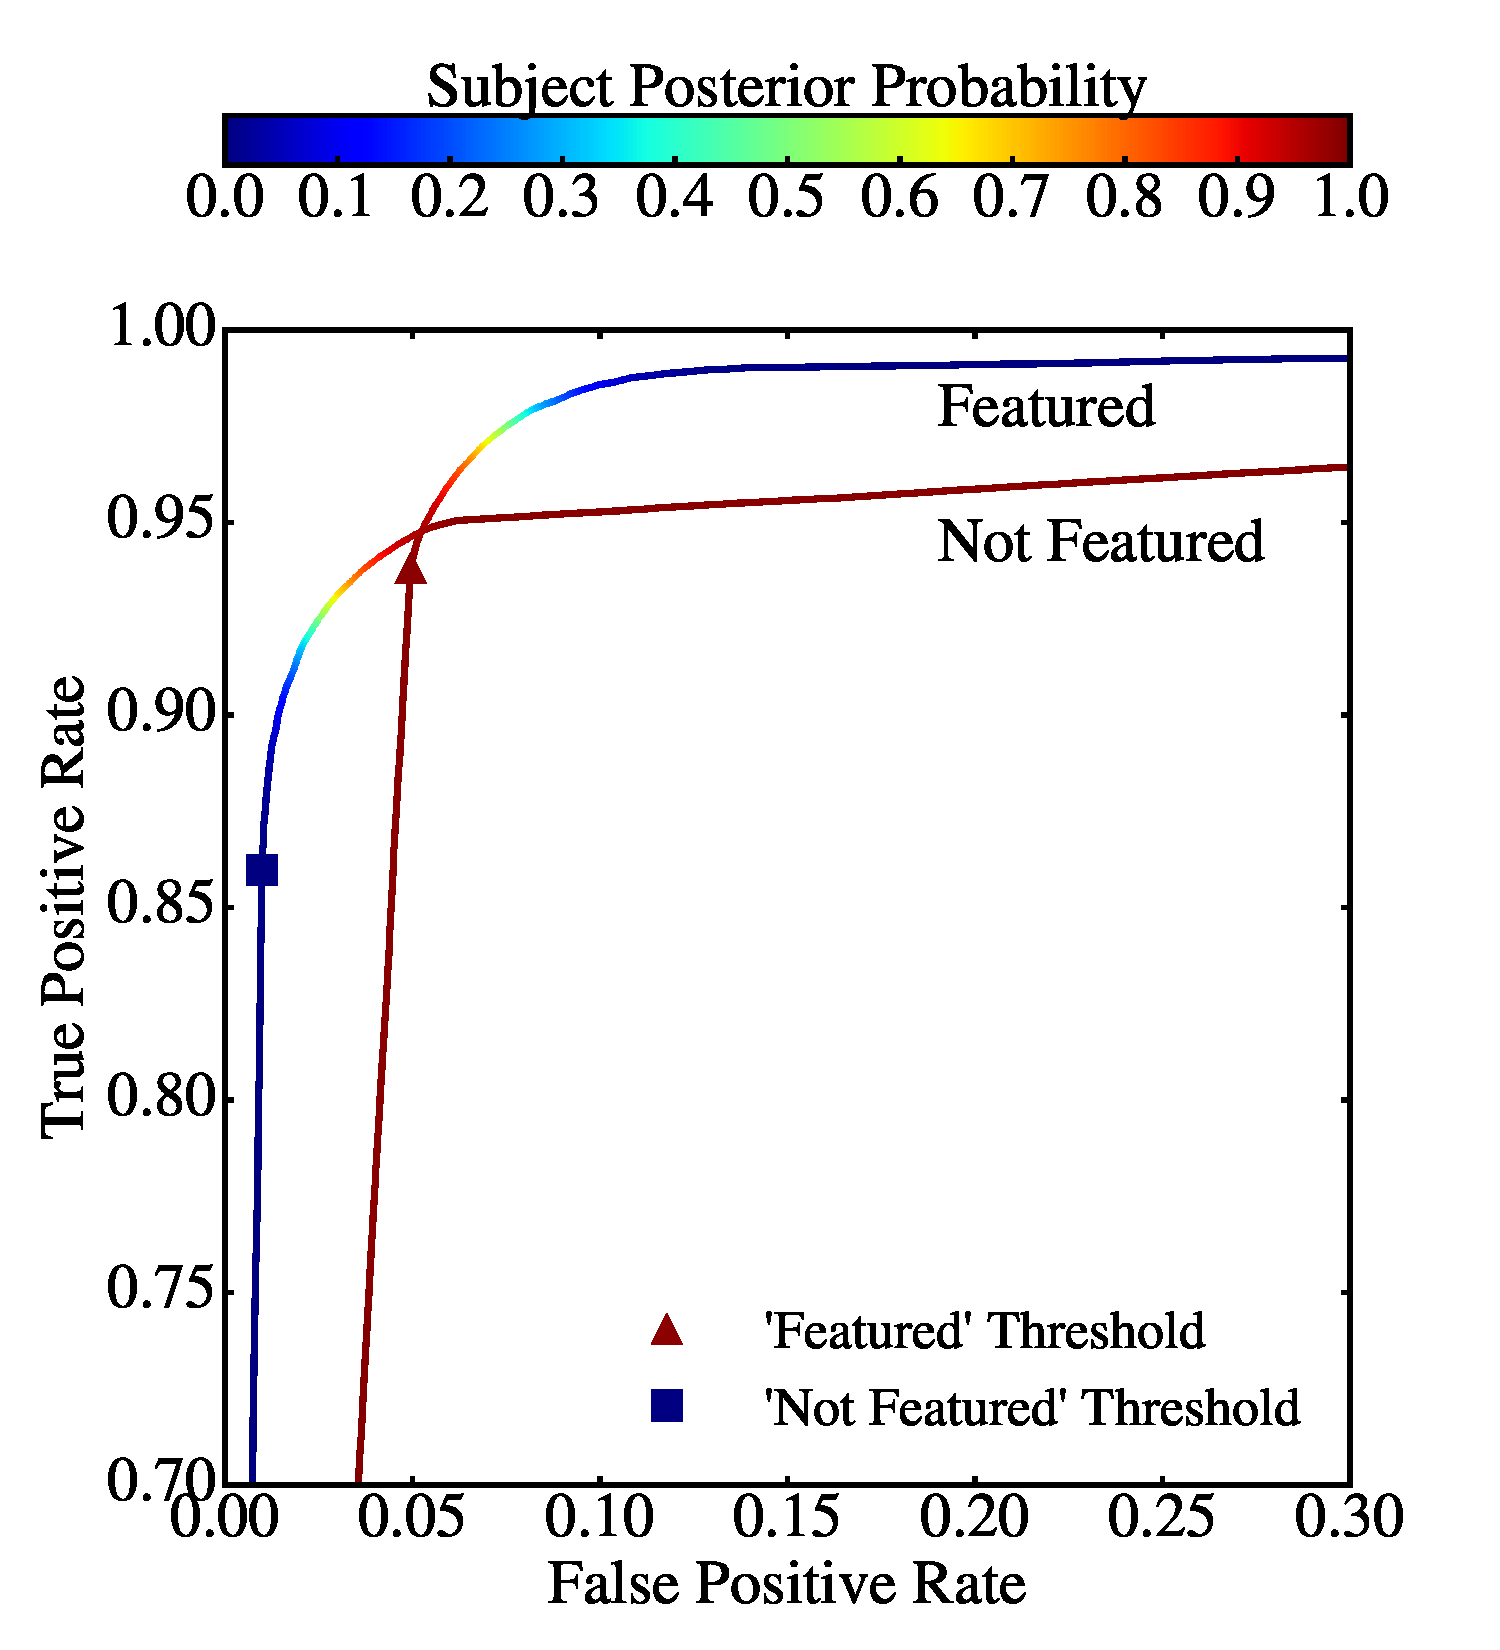
\includegraphics[width=3.08in]{Figures/human_machine/A2a.pdf}
\caption[Receivor operating characteristic curve for the chosen SWAP retirement thresholds.]{Identifying~\feat~subjects is independent of identifying~\notfeat~subjects.  Both ROC curves use all subjects processed by SWAP where the score used to create the ROC curve is simply each subject's achieved posterior probability. The Featured curve demonstrates how well we identify~\feat~subjects with a threshold of 0.99, while the Not Featured curve demonstrates how well we identify~\notfeat~subjects with a threshold of 0.004. Typically, best performance is achieved by the score associated with the upper-left-most part of the curve. Our~\feat~threshold is nearly optimal, while our~\notfeat~threshold could be improved since the blue square is not as close to the upper left hand corner as other possible values of the subject posterior.}
\label{fig: morph thresh}
\end{center}
\end{figure}

\subsection{Retirement thresholds, \tf~and~\tn.}
Retirement thresholds are directly related to the time that a subject will spend in SWAP before retirement. If we lower~\tf~(and/or raise~\tn), more subjects will be retired compared to the fiducial run as each subject will have a smaller swath of probability space in which to fluctuate before crossing one of these thresholds. On the other hand, if we raise~\tf~(and/or lower~\tn), it will take longer for subjects to cross one of these thresholds. This also increases the likelihood of some subjects never crossing either threshold, instead oscillating indefinitely through probability space.

What thresholds should one choose? To answer this question, we consider the left panel of Figure~\ref{fig: morph thresh}, which depicts the receiver operating characteristic (ROC) curve for our fiducial simulation, an illustration of performance as a function of a threshold for a binary classifier. ROC curves display the true positive rate against the false positive rate for a discriminatory threshold or score with a perfect classifier achieving 100\% true positives and no false positives. The value of the threshold optimal for predicting class labels would be that which allows the ROC curve to reach the upper-left-most point in the diagram. We have two thresholds to consider and thus we plot the curve twice: once under the assumption that ``true positives" denote correctly identified~\feat~subjects; and again under the assumption that ``true positives" instead denote correctly identified~\notfeat~subjects.  In both cases, the color of the line corresponds to the subject posterior probability. We mark the location of~\tf~$=0.99$~and~\tn~$=0.004$
from our fiducial run with a red triangle and blue square respectively. We see that~\tf~is nearly optimal but~\tn~could be improved upon. 